\documentclass[accentcolor=tud9b, colorbacktitle, inverttitle]{tudbeamer}

\usepackage[utf8]{inputenc}
\usepackage[T1]{fontenc}
\usepackage[ngerman]{babel}
\usepackage{epstopdf}
\epstopdfsetup{outdir=./graph/}
\usepackage{graphicx}
\usepackage{xcolor}
\usepackage{tikz}
\usepackage{lipsum,multicol}
% \usepackage[backend=biber]{biblatex}
% \addbibresource{References_PSBeschl_2018.bib}

% style=alphabetic, 
\usepackage{tikz}						% graphics creation environment frontend
\usepackage{tikz-cd}
\usepackage{import}
\usepackage{multicol}
\usepackage{subfig}
\usepackage[binary-units=true,exponent-product=\cdot]{siunitx}
\usepackage[siunitx, european]{circuitikz}
% 
\usepackage{pgfplots}					% graph plotting for pgf/tikz
\pgfplotsset{compat=1.12, grid style={gray,dotted}}

% \usetikzlibrary{external} %% comment out to stop externalization of tikz pictures
% \tikzexternalize[optimize=false, prefix=tikz-external/] % path to store the externalized stuff in
% \tikzset{external/system call={lualatex \tikzexternalcheckshellescape -halt-on-error-interaction=batchmode -jobname "\image" "\texsource"}, force remake = false}
% % \tikzset{external/force remake = false}
% \tikzexternalize

\graphicspath{{graph/}{../../Bericht/Inputfiles/Graphics/}{../../Bericht/Inputfiles/Graphics/Simulation/}}

\author{Julian Buschbaum, Benjamin Northe, Rainer Stellnberger}
\institute{Institut TEMF~\textbar~Fachgebiet Beschleunigertechnik}
\logo[1.5]{
\includegraphics{temf}}
\date{28. September 2018}
\title{Untersuchungen zur Impedanzreduktion an MA-Kavitäten durch Kurzschließen von Ringkernen \vspace{0.2em}}
\subtitle{Rainer Stellnberger, Julian Buschbaum, Benjamin Northe \\ {\small Betreuer: Jens Schweickhardt, M.Sc.}\vspace{-0.2em}\\\vspace{-0.7em}{\small Fachgebietsleiter: Prof. Dr.-Ing. Harald Klingbeil}}

\begin{document}

%%%%%%%%%%%%%%%%%%%%%%%%%%%%%%%%%%%%%%%%%%%%%%%%%%%%%%%%%%%%%%%%%%%%%%%%%%%%%%%%%%%%%%%%%%%%%%%%%%%%%%%%%%%%%%%%%%%%%%%%%%%%%%%%%%%
%%%%%%%%%%%%%%  TEIL1: Benjamin  %%%%%%%%%%%%%%%%%%%%%%%%%%%%%%%%%%%%%%%%%%%%%%%%%%%%%%%%%%%%%%%%%%%%%%%%%%%%%%%%%%%%%%%%%%%%%%%%%%

\begin{titleframe}
\vspace{-0.75em}
	\begin{figure}[h]
		\centering
		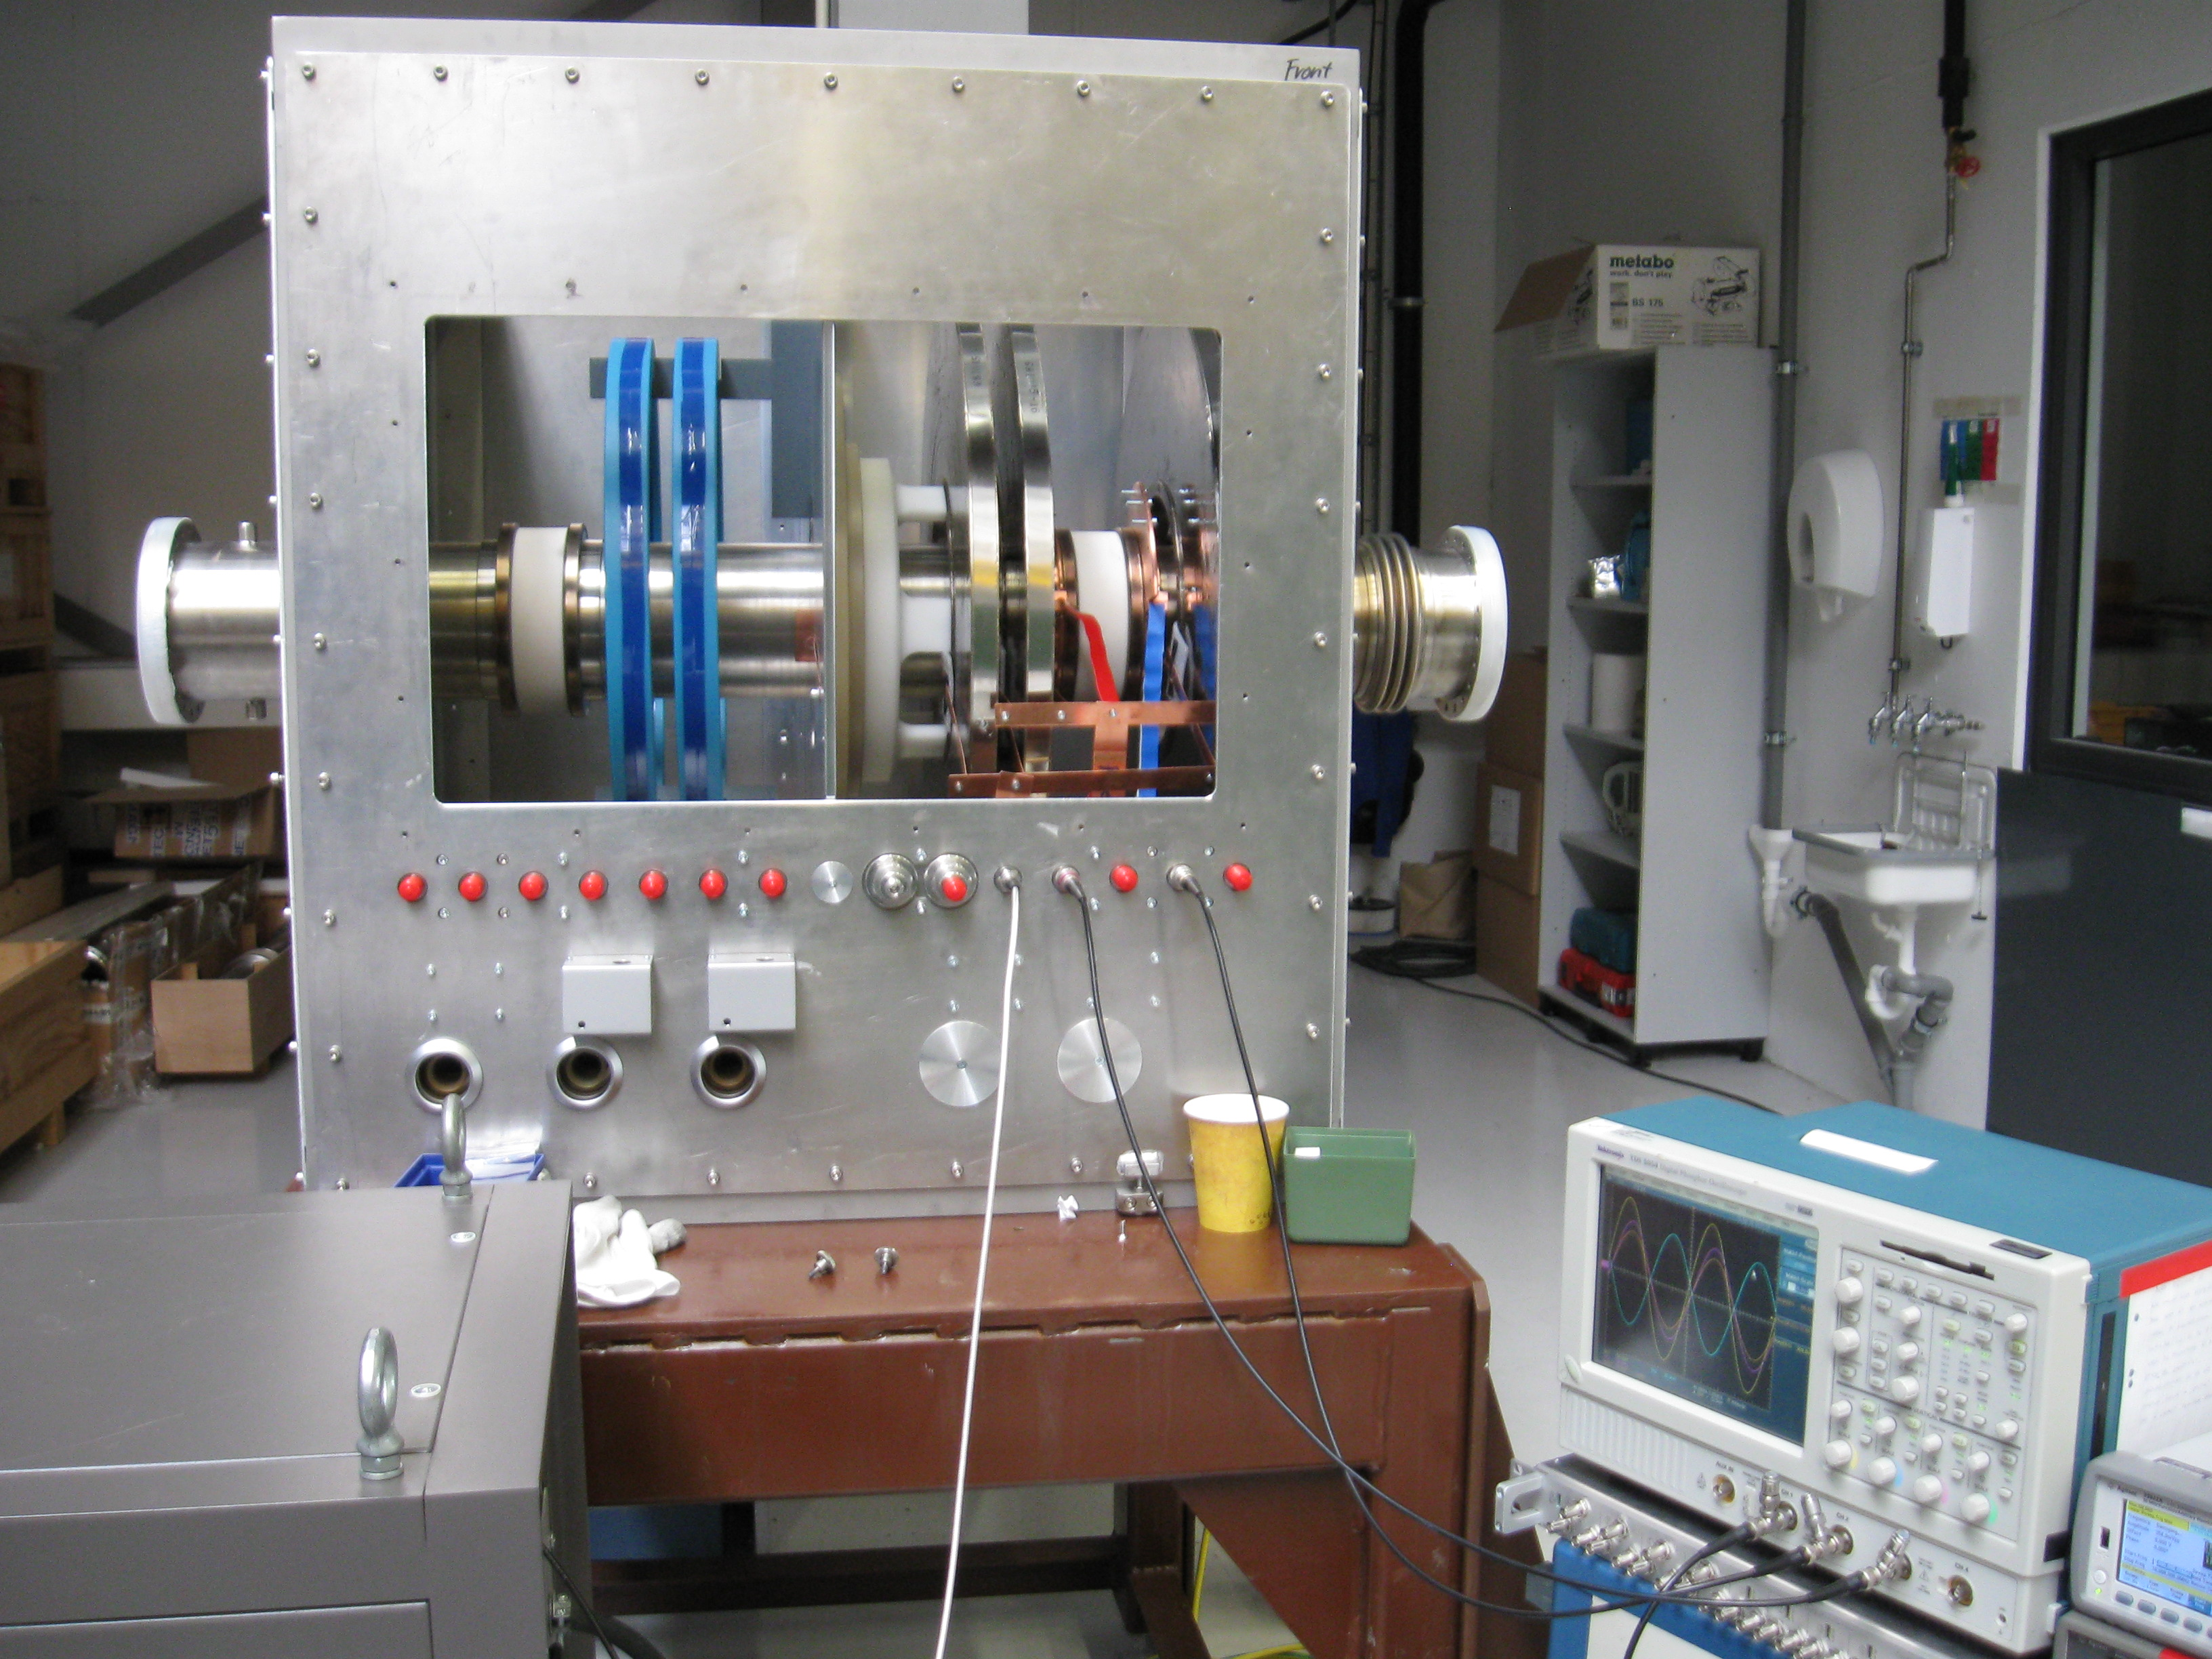
\includegraphics[width=0.6\textwidth]{Kavitaet}
	\end{figure}
\end{titleframe}




\begin{frame}\frametitle{Inhalt}
	\begin{itemize}
		\item Aufgabenstellung
		\item Der Messaufbau
		\item Simulation
		\item Gegen\"uberstellung der Messung und Simulation
		\item Auswertung der Kurzschlussanordnungen
		\item Fazit und Ausblick
	\end{itemize}
\end{frame}



\begin{frame}\frametitle{Aufgabenstellung}
\vspace{-1em}
\begin{multicols}{2}
	\begin{figure}[h]
		\centering
		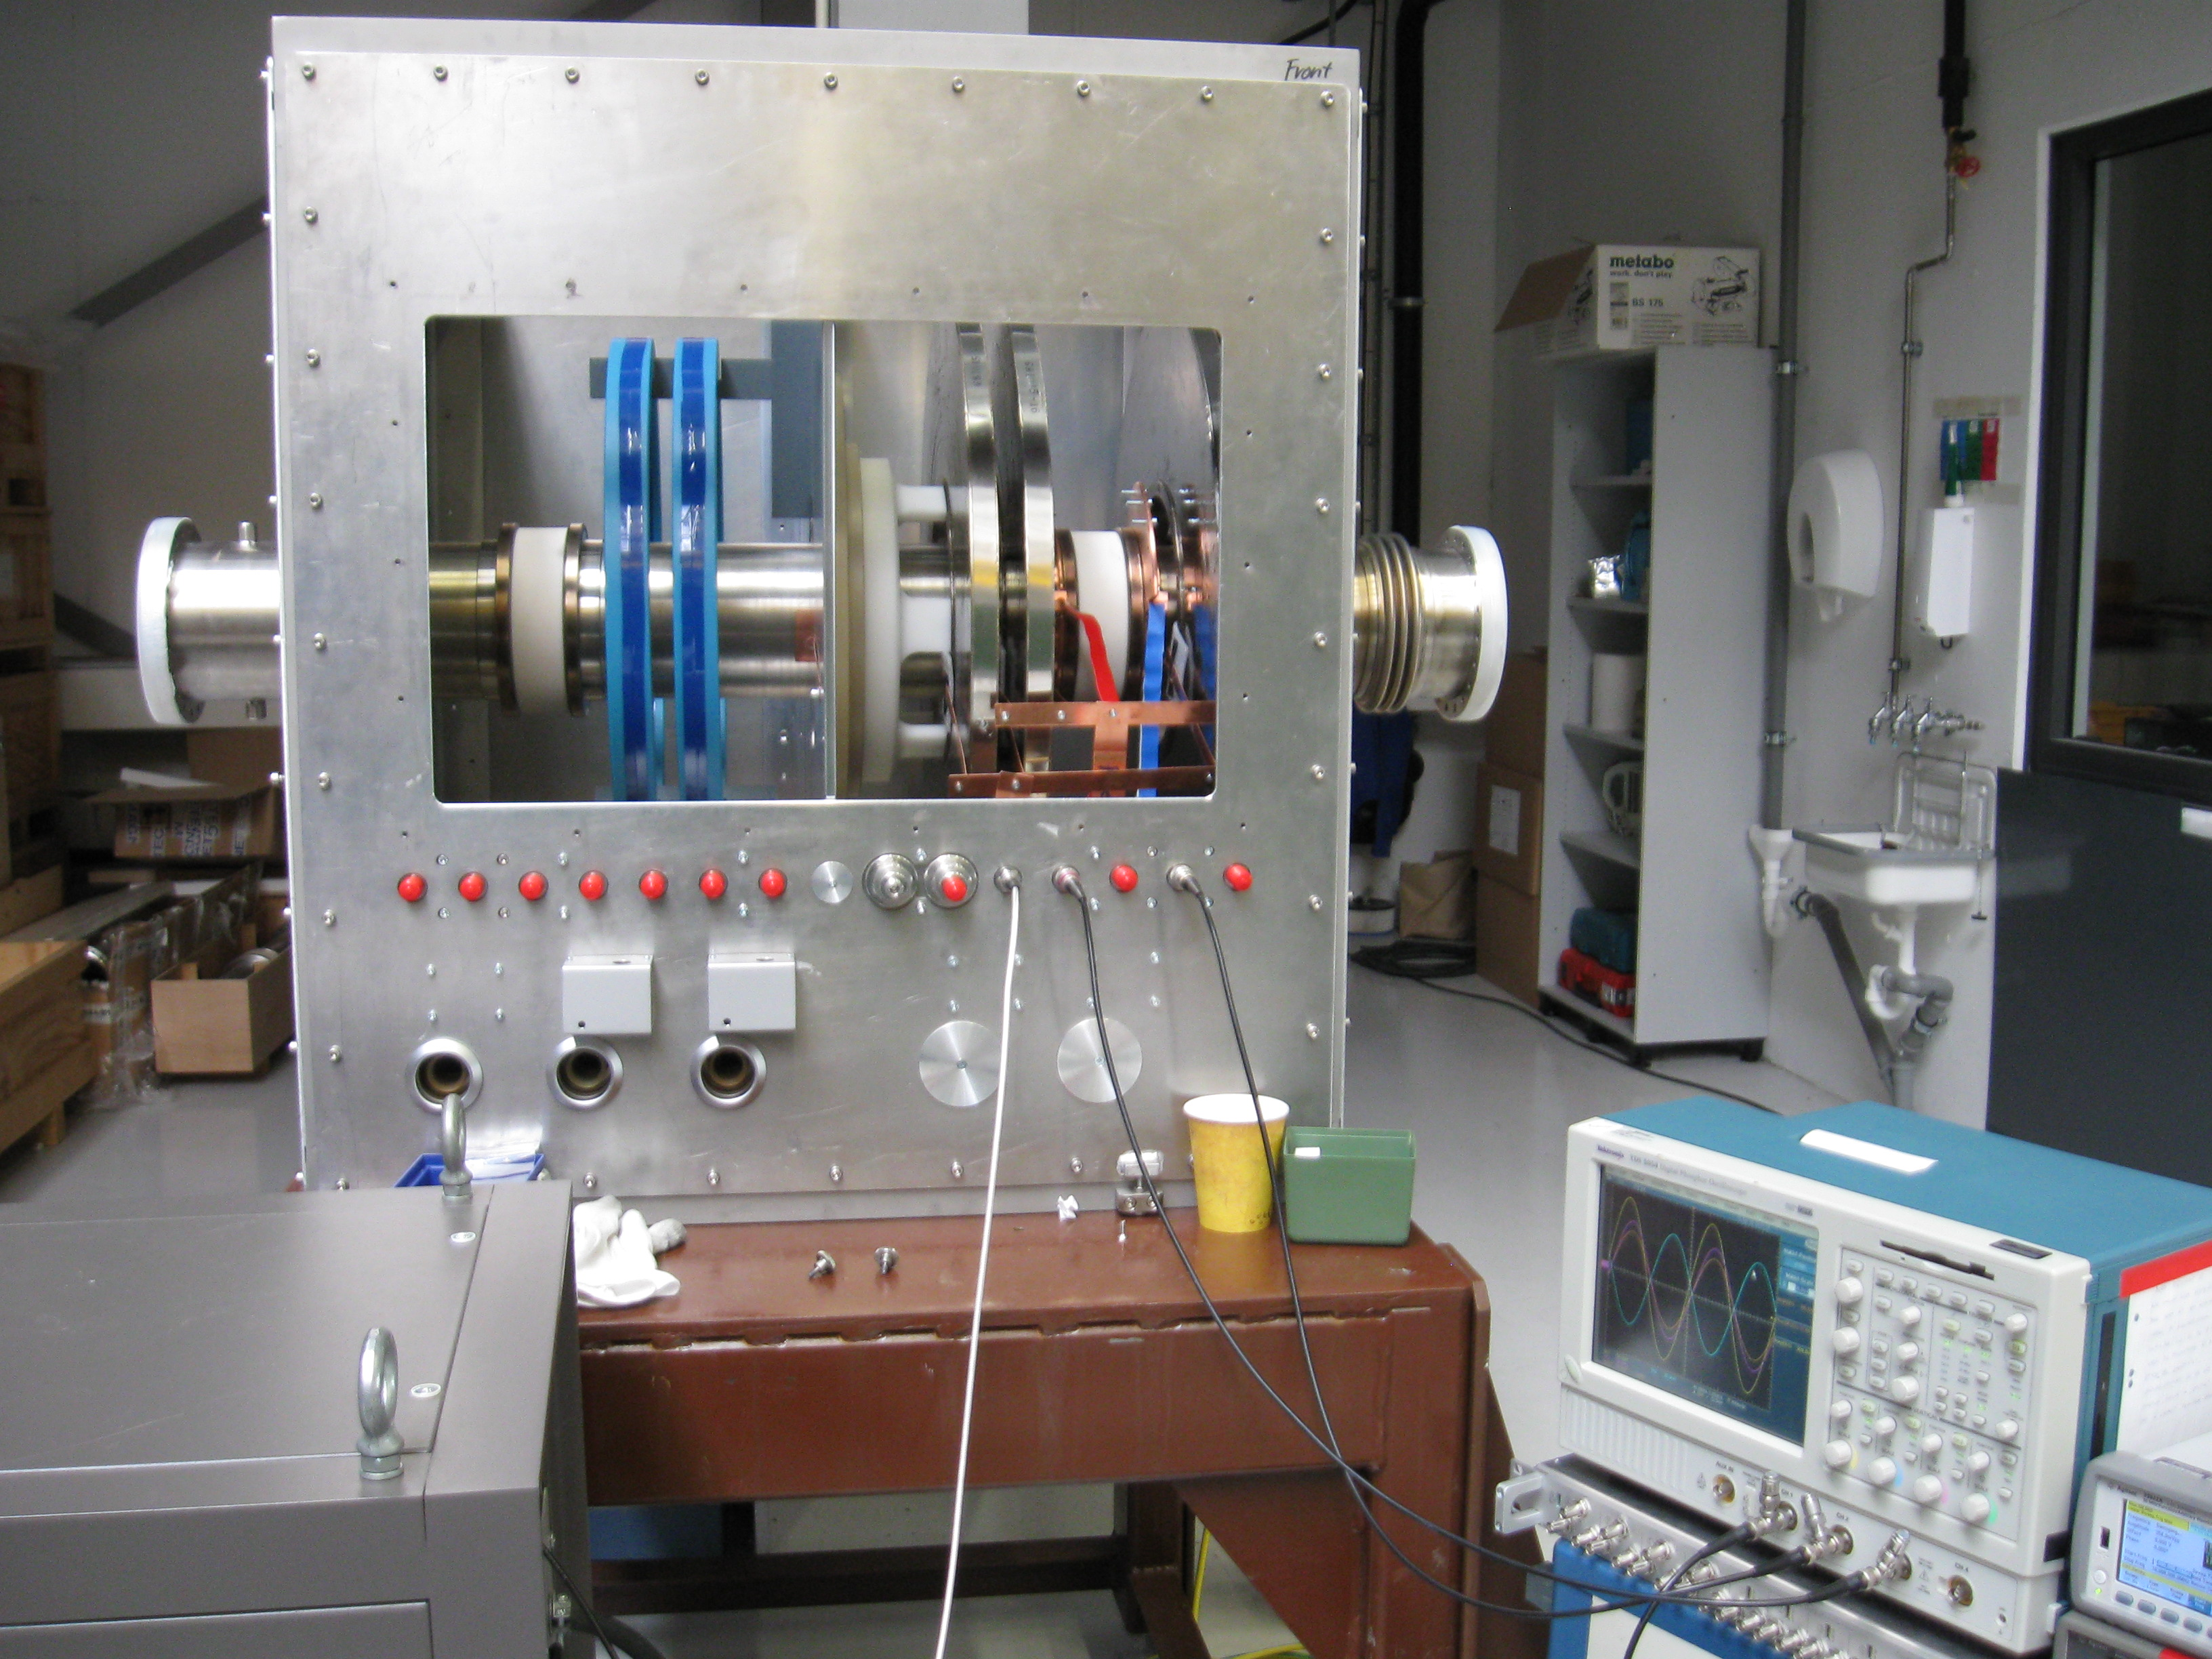
\includegraphics[width=0.5\textwidth]{Kavitaet}
	\end{figure}
	\vfill\null
	\columnbreak
	\begin{itemize}
		\item MA(Magnetic Alloy)-Ringkerne als Last der Kavit\"at
		\item Im nicht beschleunigenden Betrieb Kavit\"at m\"oglichst wenig Einfluss auf den Strahl gewünscht (geringe Shuntimpendanz)
		\item Theorie: Kurzschlussschaltung um die Ringkerne soll deren Impedanz und damit die der gesamten Kavität reduzieren
	\end{itemize}
\end{multicols}
\end{frame}


\begin{frame}\frametitle{Herangehensweise}
\begin{itemize}
	\item Parallele Messungen und Simulationen
	\item Parameter f\"ur Kurzschl\"usse abgeleitet
	\begin{itemize}
		\item Form
		\item Abmessungen
		\item Anzahl
	\end{itemize}
\end{itemize}
\end{frame}



\begin{frame}\frametitle{Die Testbox}
\vspace{-1em}
\begin{multicols}{2}
	\begin{figure}[h]
		\centering
		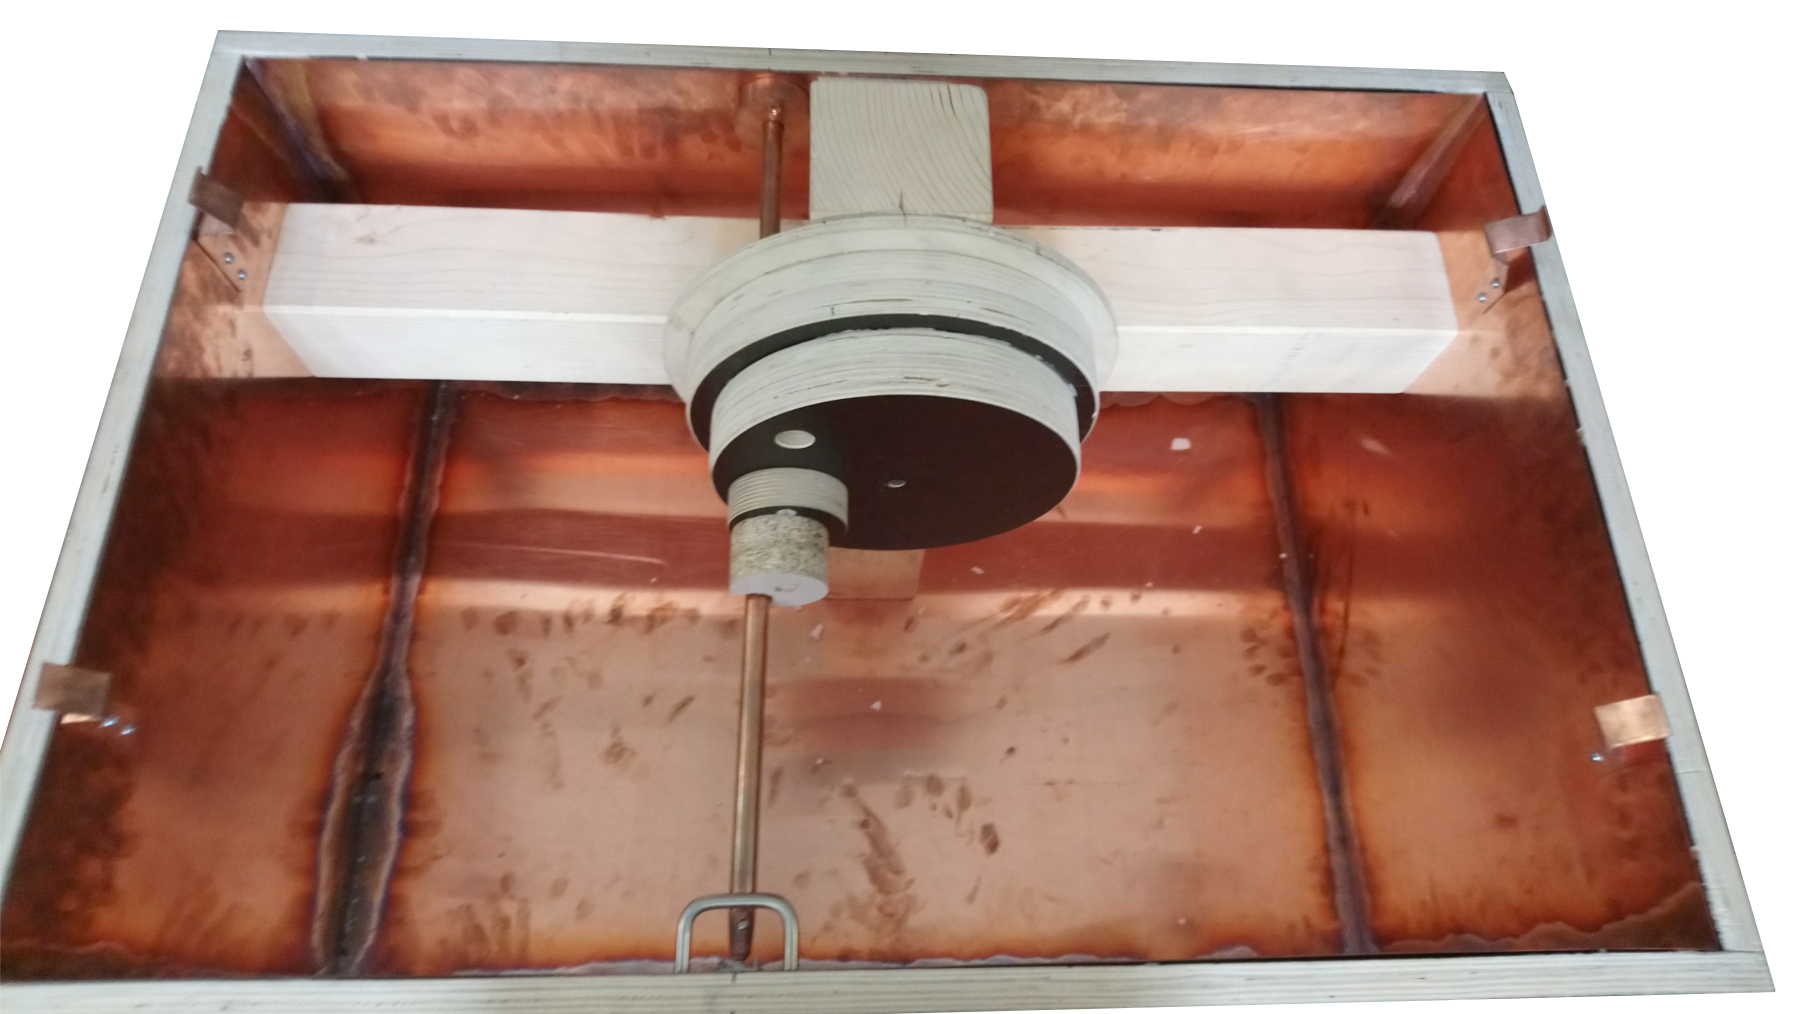
\includegraphics[width=0.5\textwidth]{boxleer}
	\end{figure}
	\vfill\null
	\columnbreak
	\begin{itemize}
		\item Innen mit Kupferblech (Dicke $\SI{1}{\milli\meter}$ ausgekleidet
		\item Holzkonstruktion als Ringkernhalterung
		\item Kupferrohr zur Einkopplung
		\begin{itemize}
			\item Am Rand der Box mit N-Steckerausgang 
		\end{itemize}
	\end{itemize}
\end{multicols}
\end{frame}


\begin{frame}\frametitle{Konstruktion der Ringkernhalterung}
\vspace{-1em}
\begin{multicols}{2}
	\begin{figure}[h]
		\centering
		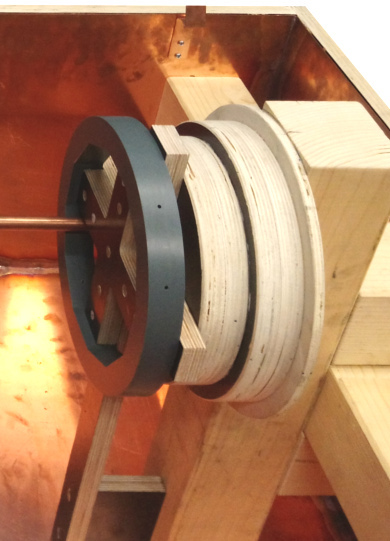
\includegraphics[width=0.35\textwidth]{BoxKreuzPolygonpraes}
	\end{figure}
	\vfill\null
	\columnbreak
	\begin{itemize}
		\item Anordnung um gew\"unschte Messungen durchzuf\"uhren
		\item Ringf\"ormige Halterung, an Innenseite Polygonzug
		\item Schraubenl\"ocher mit Gewinde in Polygon zur Fixierung
		\item Reproduzierbare Positionierung
		\item Pr\"azise Montage
	\end{itemize}
\end{multicols}
\end{frame}


\begin{frame}\frametitle{Entwurf der Kurzschlussschienen}
\vspace{-2em}
% \begin{multicols}{2}
	\begin{figure}[h]
		\flushleft
		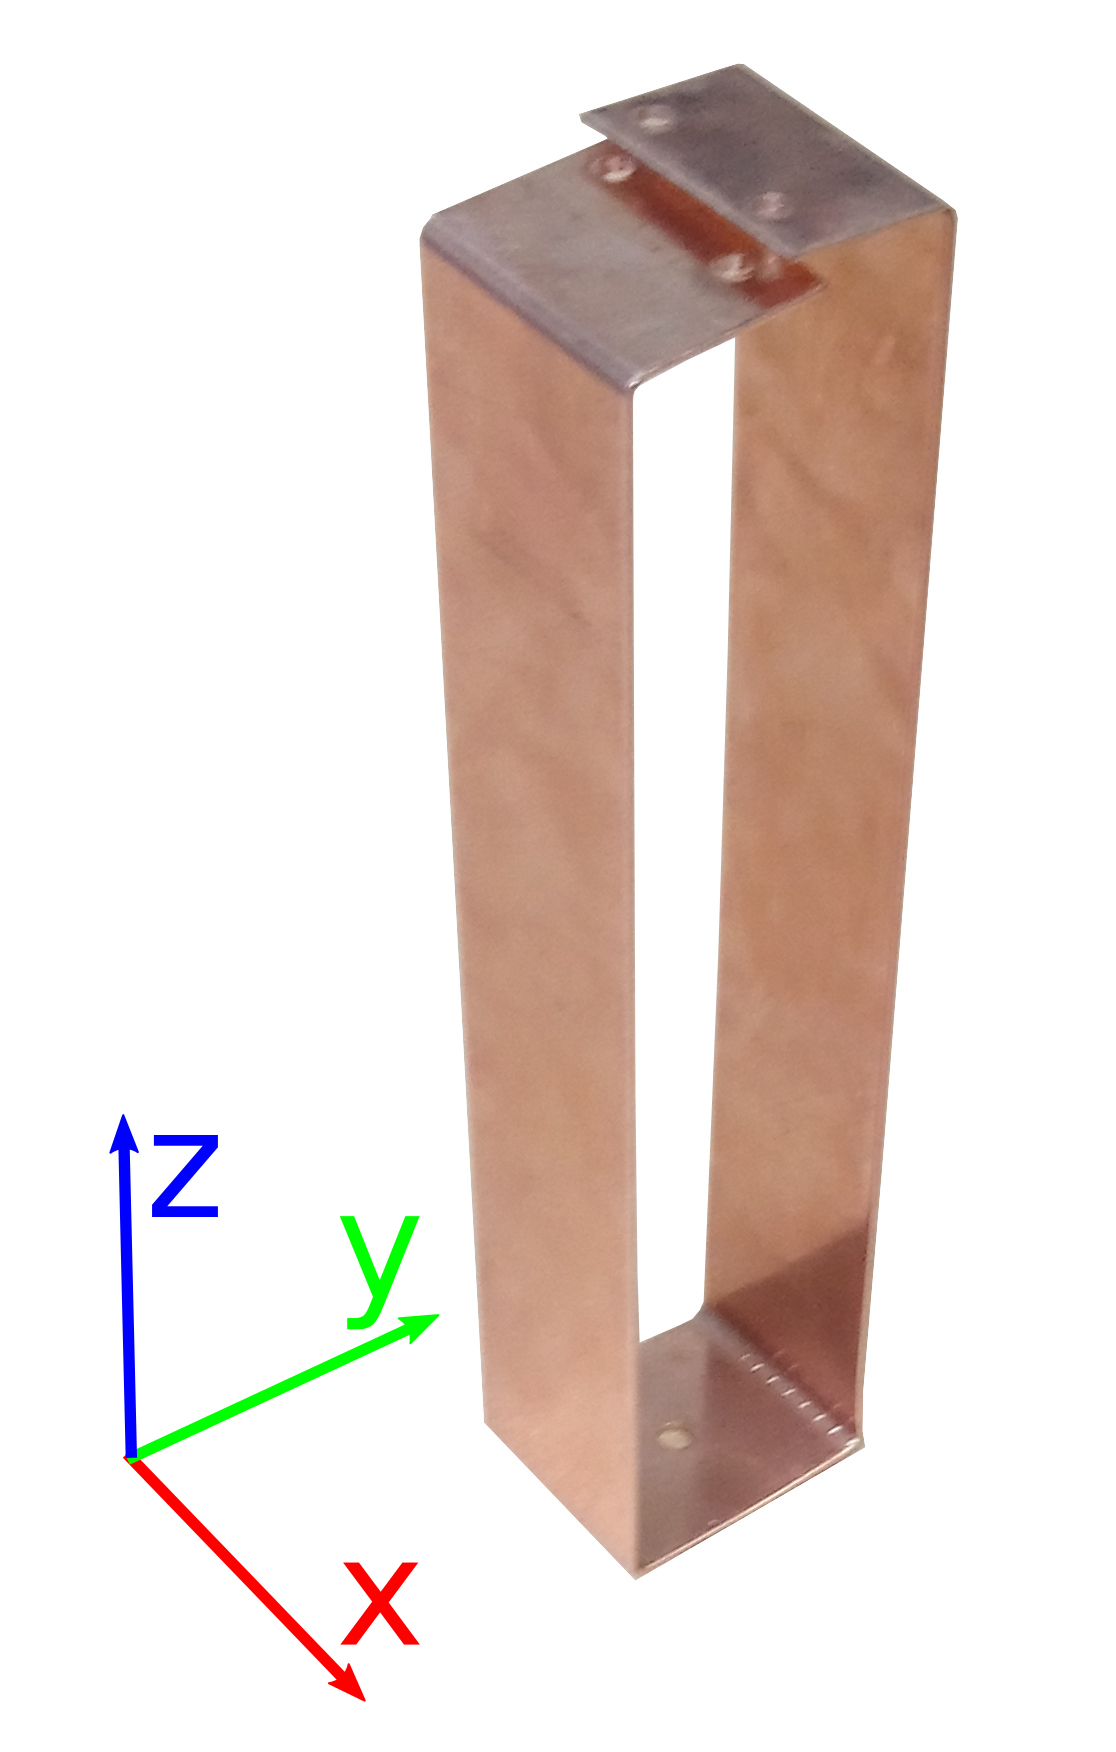
\includegraphics[width=0.28\textwidth]{KS}
	\end{figure}
% 	\vfill\null
% 	\columnbreak
\vspace{-0.45\textwidth}
\hspace{0.3\textwidth}
\begin{minipage}[t]{0.6\textwidth}
	\begin{itemize}
		\item Lochung im unteren Teil zur Montage
		\item Lochungen im oberen Teil zur Kontaktherstellung
		\item Mehrere Variationsparameter der Form gefertigt:
% 		\begin{itemize}
% 			\item L\"ange der Kurzschl\"usse in z-Richtung
% 			\item Breite der Kurzschl\"usse in x-Richtung
% 			\item Blechdicke der K\"urzschl\"usse
% 		\end{itemize}
	\end{itemize}
\end{minipage}	
	\begin{minipage}[t]{0.6\textwidth}
\vspace{1em}
\hspace{0.55\textwidth}
{\small
	\begin{tabular}{ | l | l |  l | l | }
		\hline
		\multicolumn{3}{|l|}{Kurzschlussform} & Anzahl \\ \cline{0-2}
		L\"ange in z & Breite in x & Blechdicke & Kurzschl\"usse \\\hline
		$\SI{160}{\milli\meter}$ & $\SI{30}{\milli\meter}$ & $\SI{1}{\milli\meter}$ & 1-8 \\
		$\SI{160}{\milli\meter}$ & $\SI{20}{\milli\meter}$ & $\SI{1}{\milli\meter}$ & 1-2 \\
		$\SI{160}{\milli\meter}$ & $\SI{50}{\milli\meter}$ & $\SI{1}{\milli\meter}$ & 1-2 \\
		$\SI{200}{\milli\meter}$ & $\SI{30}{\milli\meter}$ & $\SI{1}{\milli\meter}$ & 1-2 \\
		$\SI{250}{\milli\meter}$ & $\SI{30}{\milli\meter}$ & $\SI{1}{\milli\meter}$ & 1-2 \\
		$\SI{160}{\milli\meter}$ & $\SI{30}{\milli\meter}$ & $\SI{2}{\milli\meter}$ & 1-2 \\ \hline
	\end{tabular}}
\end{minipage}
	\vfill\null
% \end{multicols}
\end{frame}


%%%%%%%%%%%%%%%%%%%%%%%%%%%%%%%%%%%%%%%%%%%%%%%%%%%%%%%%%%%%%%%%%%%%%%%%%%%%%%%%%%%%%%%%%%%%%%%%%%%%%%%%%%%%%%%%%%%%%%%%%%%%%%%%%%%
%%%%%%%%%%%%%%  TEIL2: Julian  %%%%%%%%%%%%%%%%%%%%%%%%%%%%%%%%%%%%%%%%%%%%%%%%%%%%%%%%%%%%%%%%%%%%%%%%%%%%%%%%%%%%%%%%%%%%%%%%%%%%



\begin{frame}\frametitle{Messaufbau}
\vspace{-1em}
\begin{multicols}{2}
	\begin{figure}[h]
		\centering
		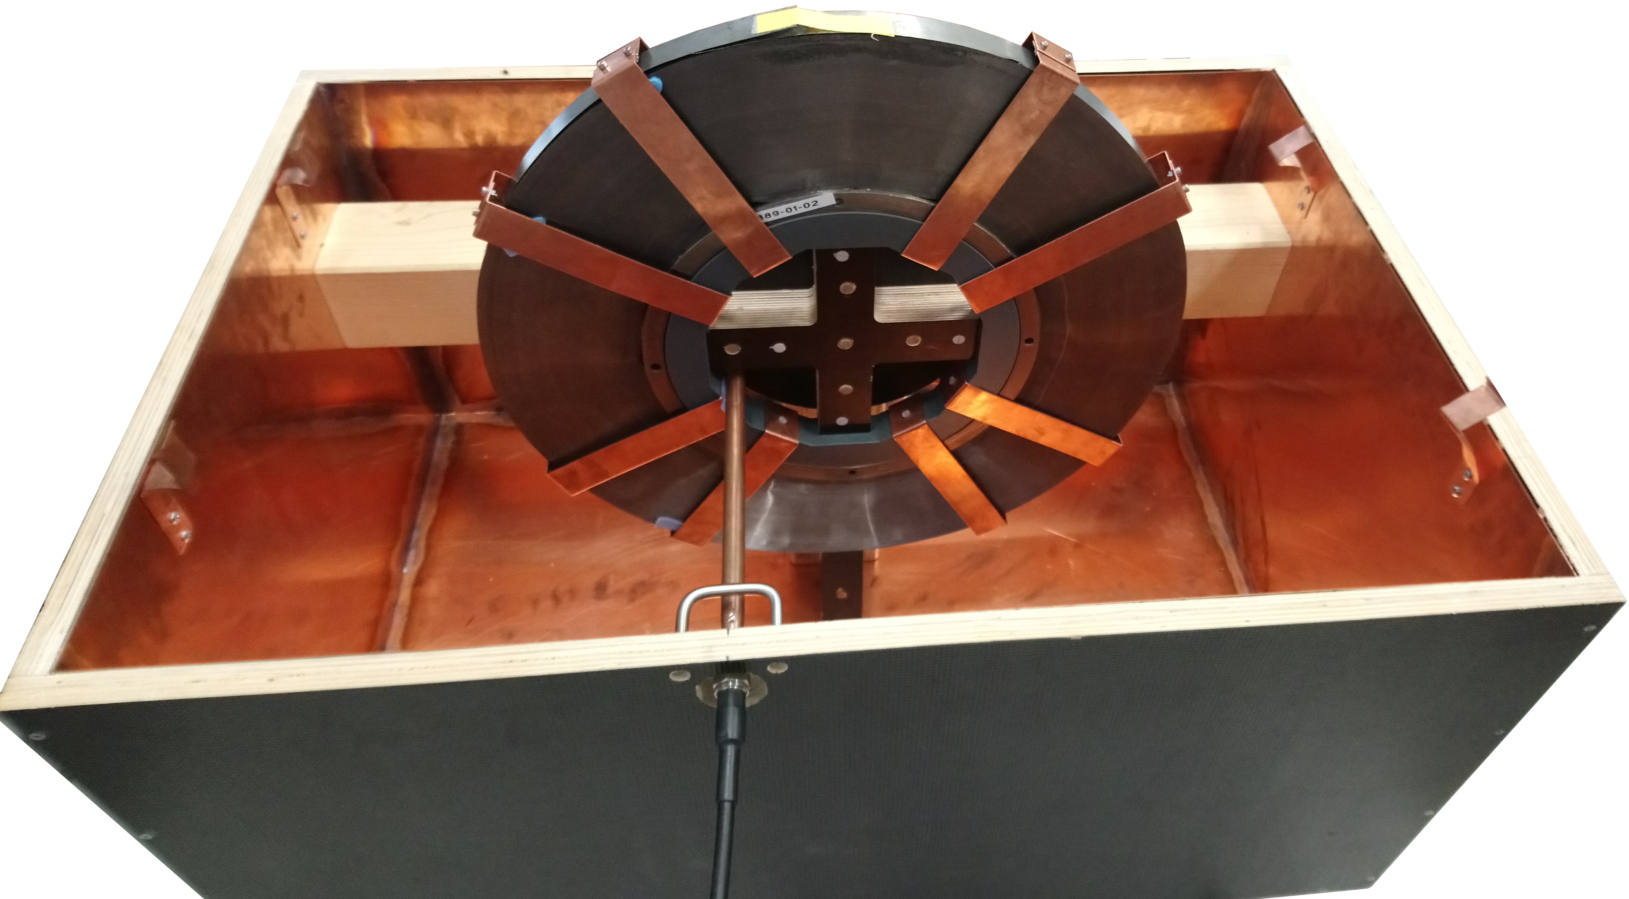
\includegraphics[width=0.38\textwidth]{BoxKreuzPolygonRK8Ks}
	\end{figure}
	\begin{figure}[h]
		\centering
		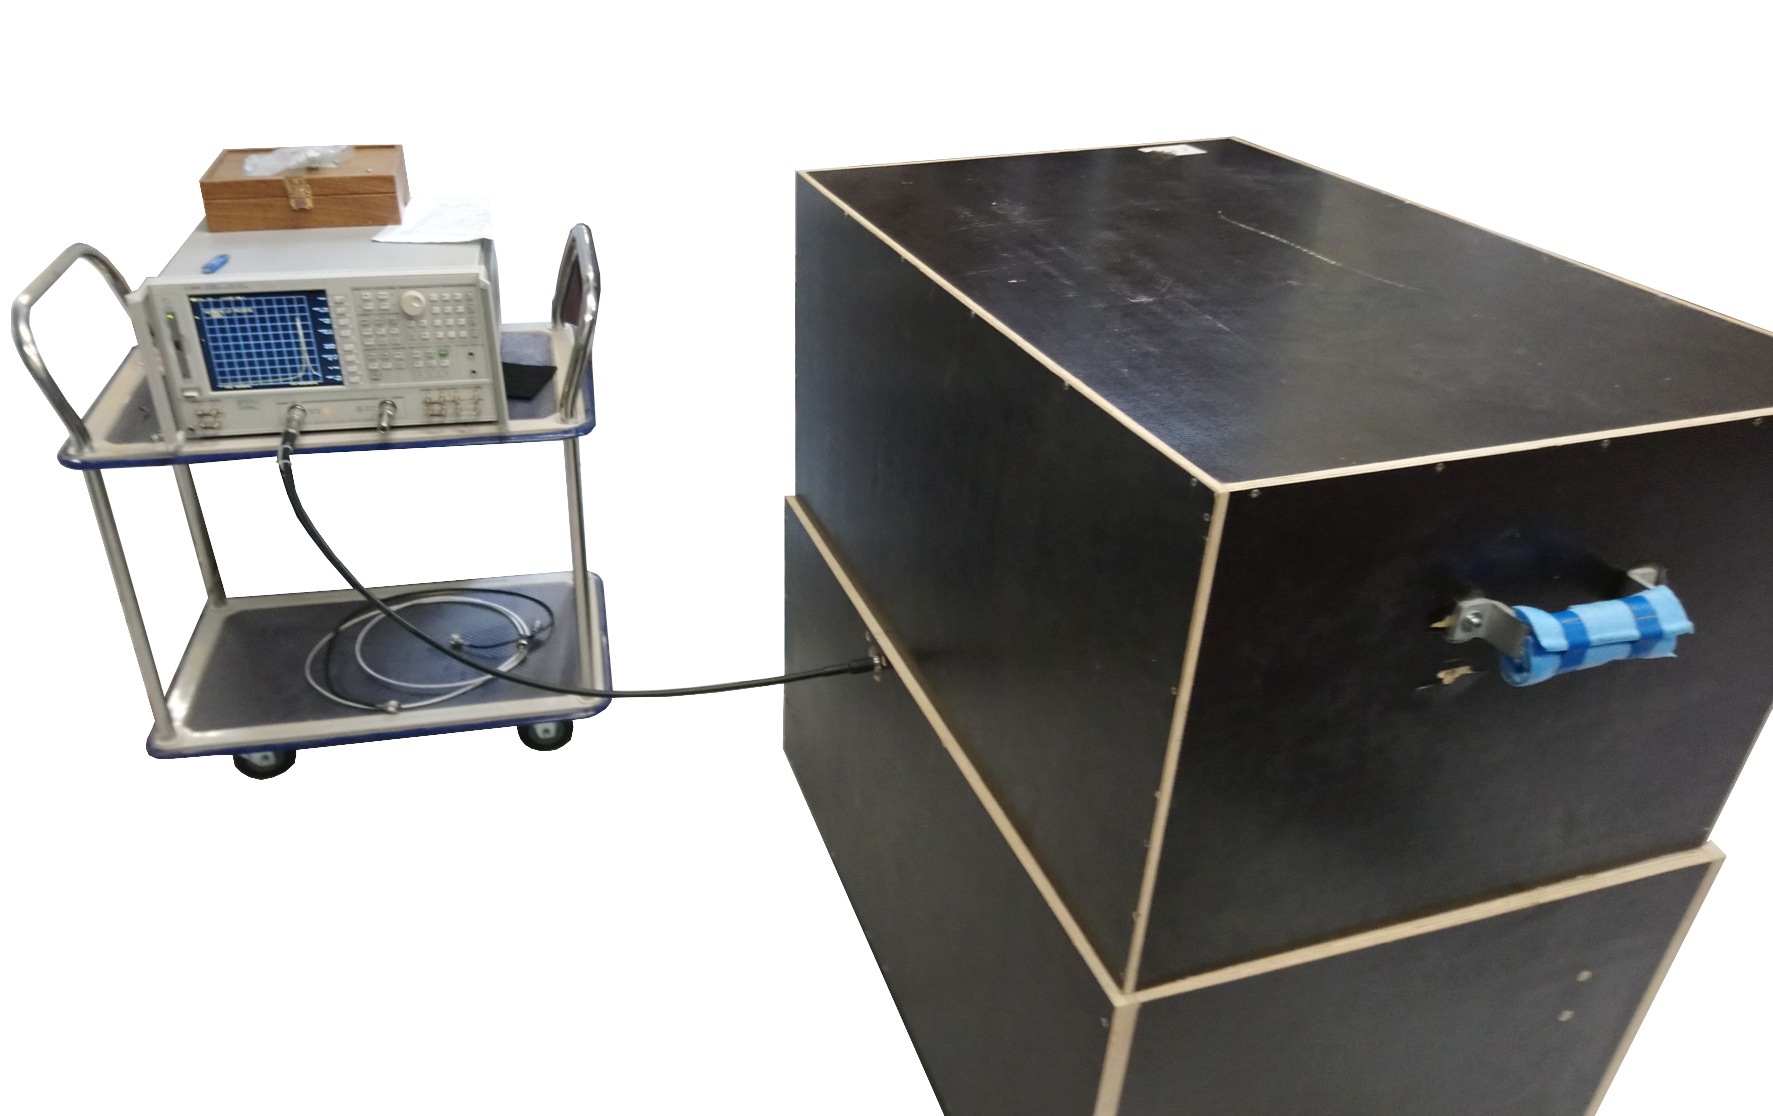
\includegraphics[width=0.38\textwidth]{messstand}
	\end{figure}
	\vfill\null
	\columnbreak
	\begin{itemize}
		\item Montage von 1-8 Kurzschl\"ussen
		\item Verschluss der Box (St\"oreinffl\"usse minimeren)
		\item Messung mittels Netzwerk-Analysator: $S_{11}$ Parameter gemessen und daraus $Z_{refl}$ der Anordnung bestimmt
	\end{itemize}
\end{multicols}
\end{frame}


% \begin{frame}\frametitle{Durchgef\"uhrte Messungen}
% \vspace{-1em}
% \begin{minipage}[t]{0.3\textwidth}
% 	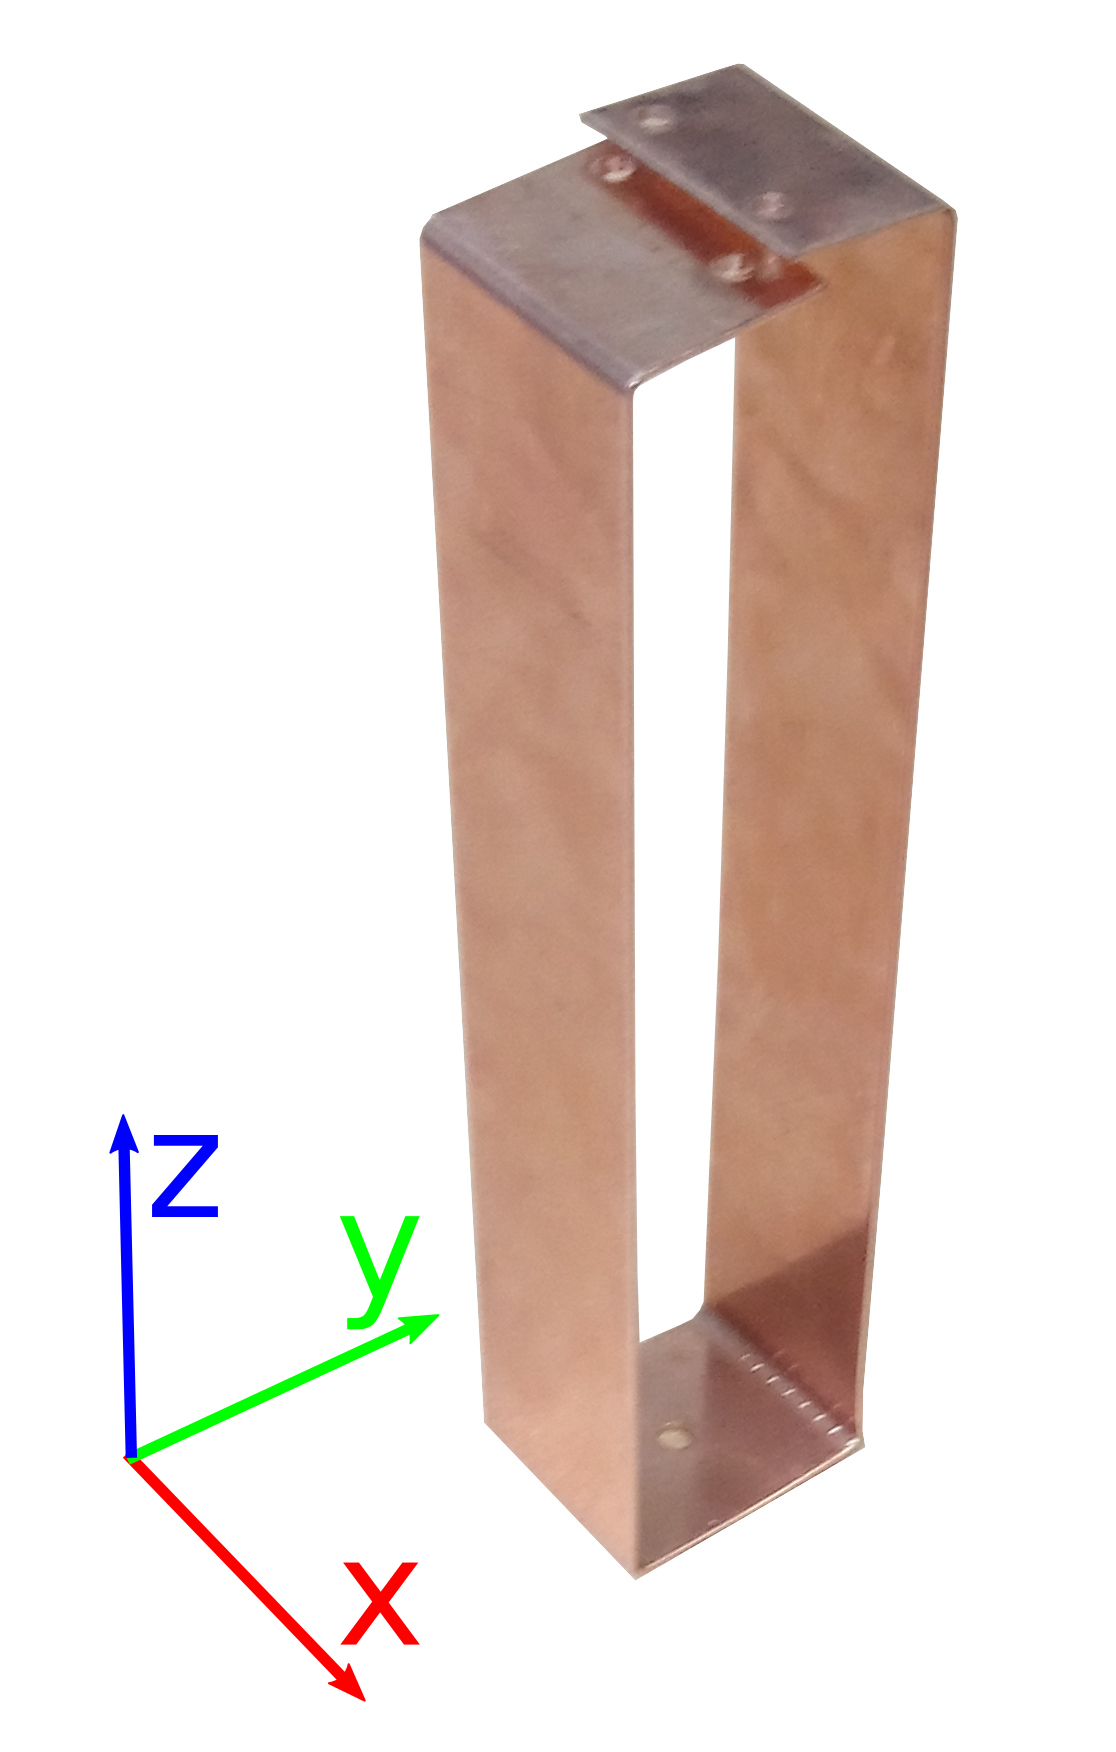
\includegraphics[width=\textwidth]{KS}
% \end{minipage}
% \begin{minipage}[t]{0.6\textwidth}
% \vspace{-0.75\textwidth}
% 	\begin{tabular}{ | l | l |  l | l | }
% 		\hline
% 		\multicolumn{3}{|l|}{Kurzschlussform} & Anzahl \\ \cline{0-2}
% 		L\"ange in z & Breite in x & Blechdicke & Kurzschl\"usse \\\hline
% 		$\SI{160}{\milli\meter}$ & $\SI{30}{\milli\meter}$ & $\SI{1}{\milli\meter}$ & 1-8 \\
% 		$\SI{160}{\milli\meter}$ & $\SI{20}{\milli\meter}$ & $\SI{1}{\milli\meter}$ & 1-2 \\
% 		$\SI{160}{\milli\meter}$ & $\SI{50}{\milli\meter}$ & $\SI{1}{\milli\meter}$ & 1-2 \\
% 		$\SI{200}{\milli\meter}$ & $\SI{30}{\milli\meter}$ & $\SI{1}{\milli\meter}$ & 1-2 \\
% 		$\SI{250}{\milli\meter}$ & $\SI{30}{\milli\meter}$ & $\SI{1}{\milli\meter}$ & 1-2 \\
% 		$\SI{160}{\milli\meter}$ & $\SI{30}{\milli\meter}$ & $\SI{2}{\milli\meter}$ & 1-2 \\ \hline
% 	\end{tabular}
% \end{minipage}
% \end{frame}


\begin{frame}\frametitle{RLC-Ersatzschaltbild der Testbox mit Ringkern}
\begin{figure}[htb]
	\centering
	\begin{tikzpicture}
	\node[above] at (-0.25,1.6) {$Z_{ges}$};
	\draw (-0.5,1.4) -- (0.1,1.4);
	\draw (-0.5,1.6) -- (0.1,1.6);
	\path[fill=black, draw=black]
	(0.1,1.3)  -- (0.1,1.7)  -- (0.5,1.5) --  (0.1,1.3);
	\begin{circuitikz}
	\draw
	(2,0) to [resistor =$R_{box}$] (2,3)
	(5,0) to [C, l=$C_{box}$] (5,3)
	(5,3) to [L, l=$L_{box}$] (9,3)
	(9,3) to [short, *-] (10,3)
	(9,0) to [short, *-] (10,0)
	(10,3) to [resistor =$Z_{rk}$] (10,0)
	(0,3) to [short, *-] (5,3)
	(0,0) to [short, *-] (5,0)
	(8,3) to [short, -*] (9,3)
	(5,0) to [short, -*] (9,0);
	% 		(0,0) to [short, *- , i_=$I_5$] (1.5,-2);
	\end{circuitikz}
	\end{tikzpicture}
\end{figure}
\end{frame}



\begin{frame}\frametitle{Simulation}
\vspace{-1em}
\begin{multicols}{2}
\begin{figure}[h]
	\centering
	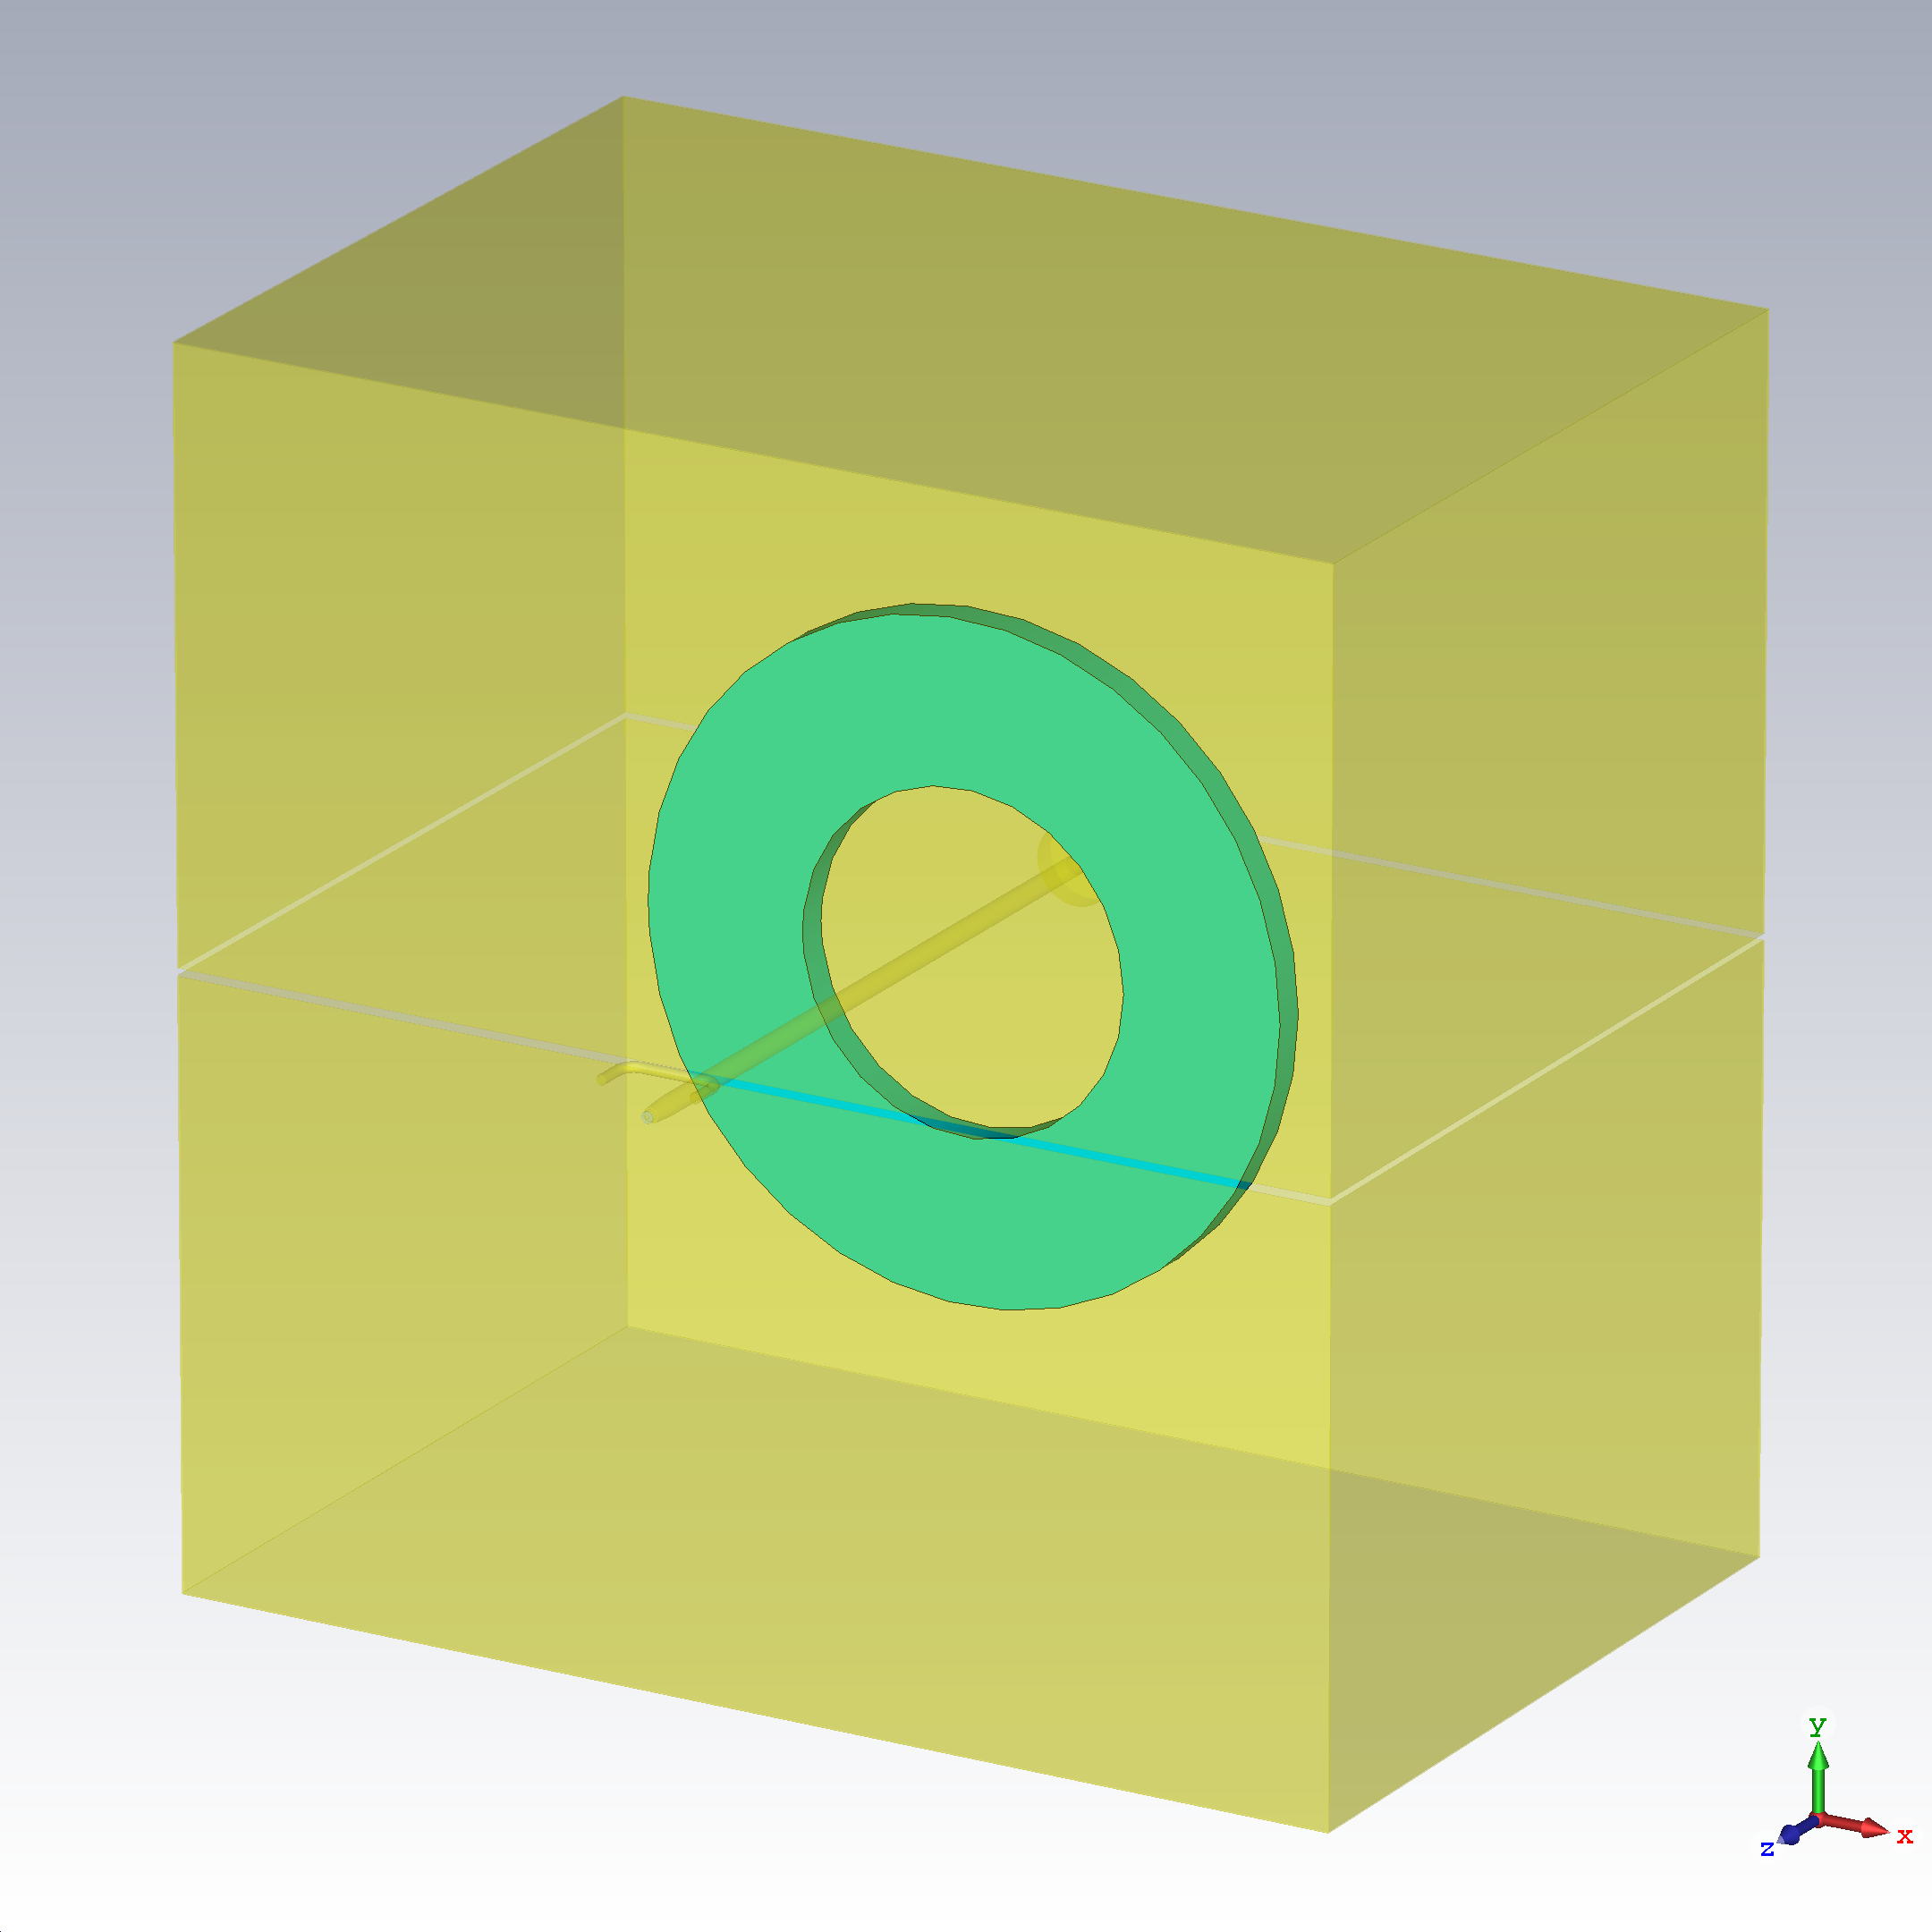
\includegraphics[width=0.48\textwidth]{BoxRK}
\end{figure}
\vfill\null
\columnbreak
\begin{itemize}
	\item Erweiterung des Modells von Denys Bast
	\item Zur Kreuzvalidierung der Ergebnisse
	\item Einfache Methode weitere Anordnungen zu testen
\end{itemize}
\end{multicols}
\end{frame}


\begin{frame}\frametitle{Realit\"atsgetreue Anpassungen der Simulation}
\vspace{-1em}
\begin{multicols}{2}
\begin{figure}[h]
	\centering
	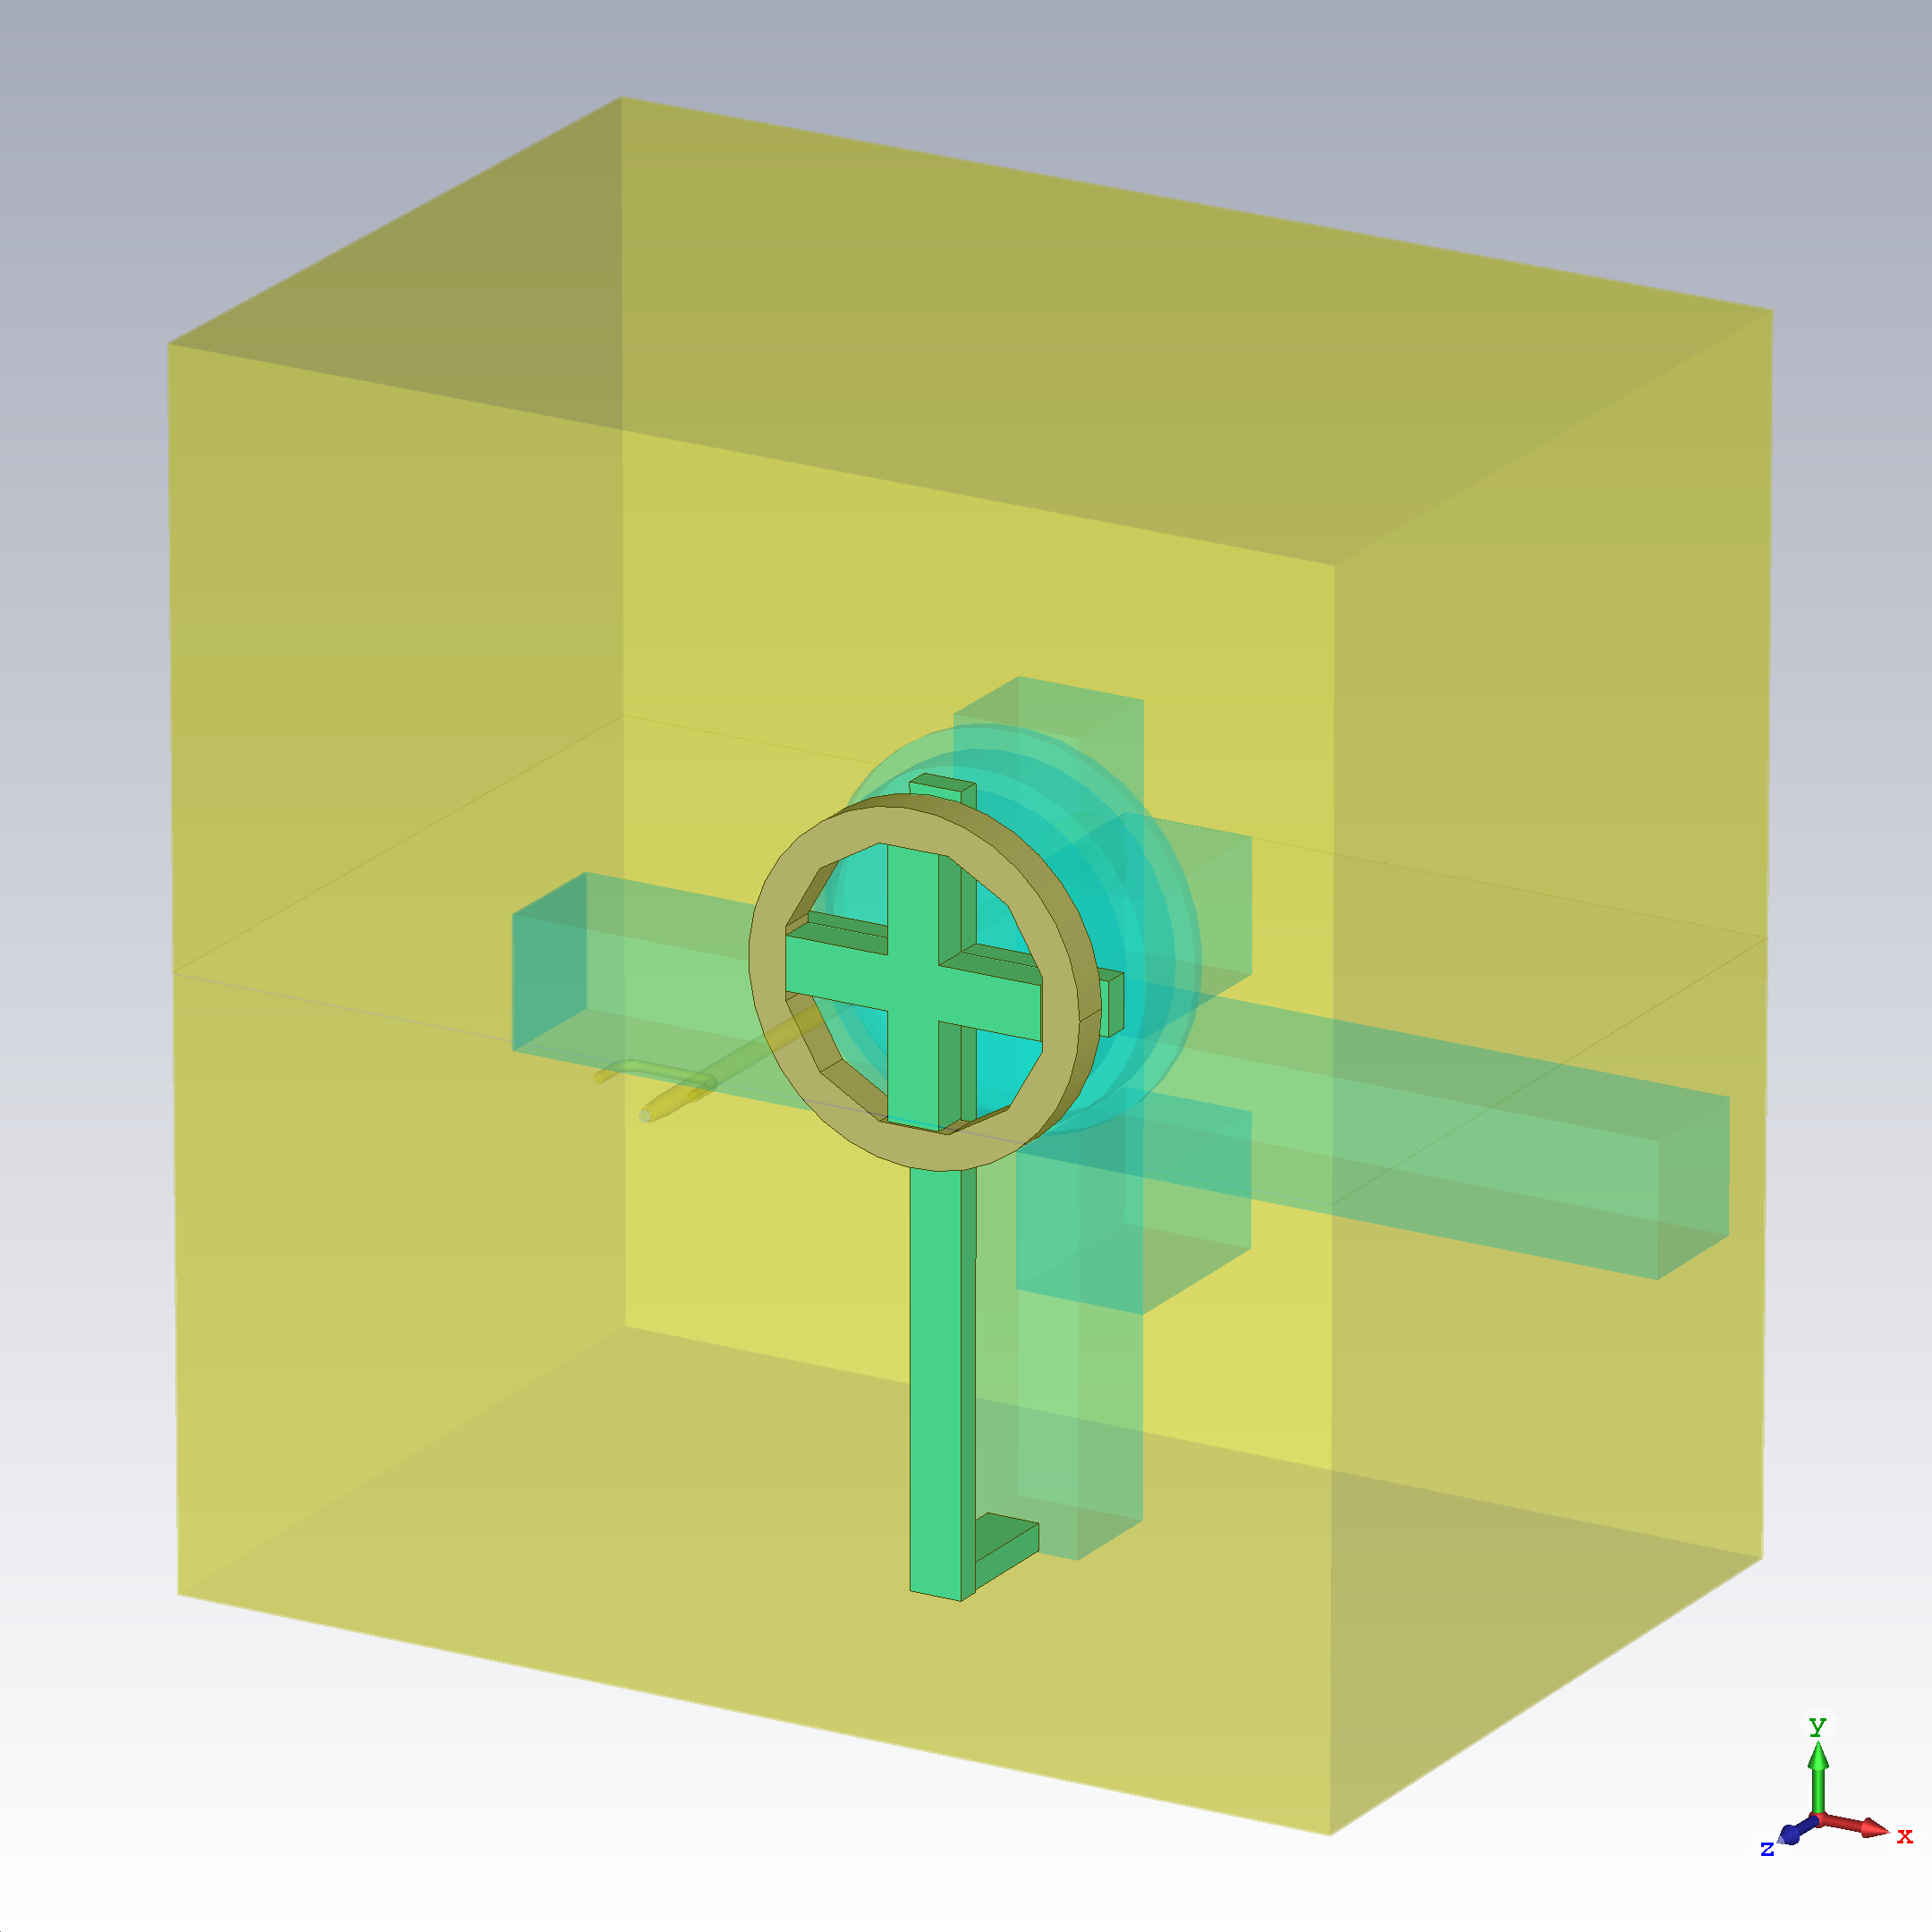
\includegraphics[width=0.48\textwidth]{KreuzPolygon}
\end{figure}
\vfill\null
\columnbreak
\begin{itemize}
	\item Einbau von Holzkonstruktion und Ringkernhalterung in Simulationsmodell
	\item Mehr F\"ullstoff in der Testbox:
	\begin{itemize}
		\item Geringere Resonanzfrequenz
		\item H\"ohere Impedanz im niedrigen Frequenzbereich
	\end{itemize}
	\item Ziel:
	\begin{itemize}
		\item Bessere Approximation des realen Aufbaus
		\item Messfehler evaluieren oder ausschlie\ss{}en
	\end{itemize}
\end{itemize}
\vfill\null
\end{multicols}
\end{frame}


% kann eventuell auch raus
\begin{frame}\frametitle{Ringkernmodellierung}
\begin{itemize}
	\item Ringkernmaterial anhand von Messung modelliert
	\item Dissipatives, komplexes $\underline{\mu}_r$
	\item Material in CST \"ubergeben und f\"ur Simulation verwendet
\end{itemize}
\end{frame}


% % Kann eher in den Anhang, lasse das erstmal raus
% \begin{frame}\frametitle{Simulationsdurchf\"uhrung}
% 
% \end{frame}



\begin{frame}\frametitle{Gegen\"uberstellung der Simulations- und Messergebnisse (ohne Kurzschl\"usse)}
\vspace{-1em}
\begin{figure}[h]
	\centering
	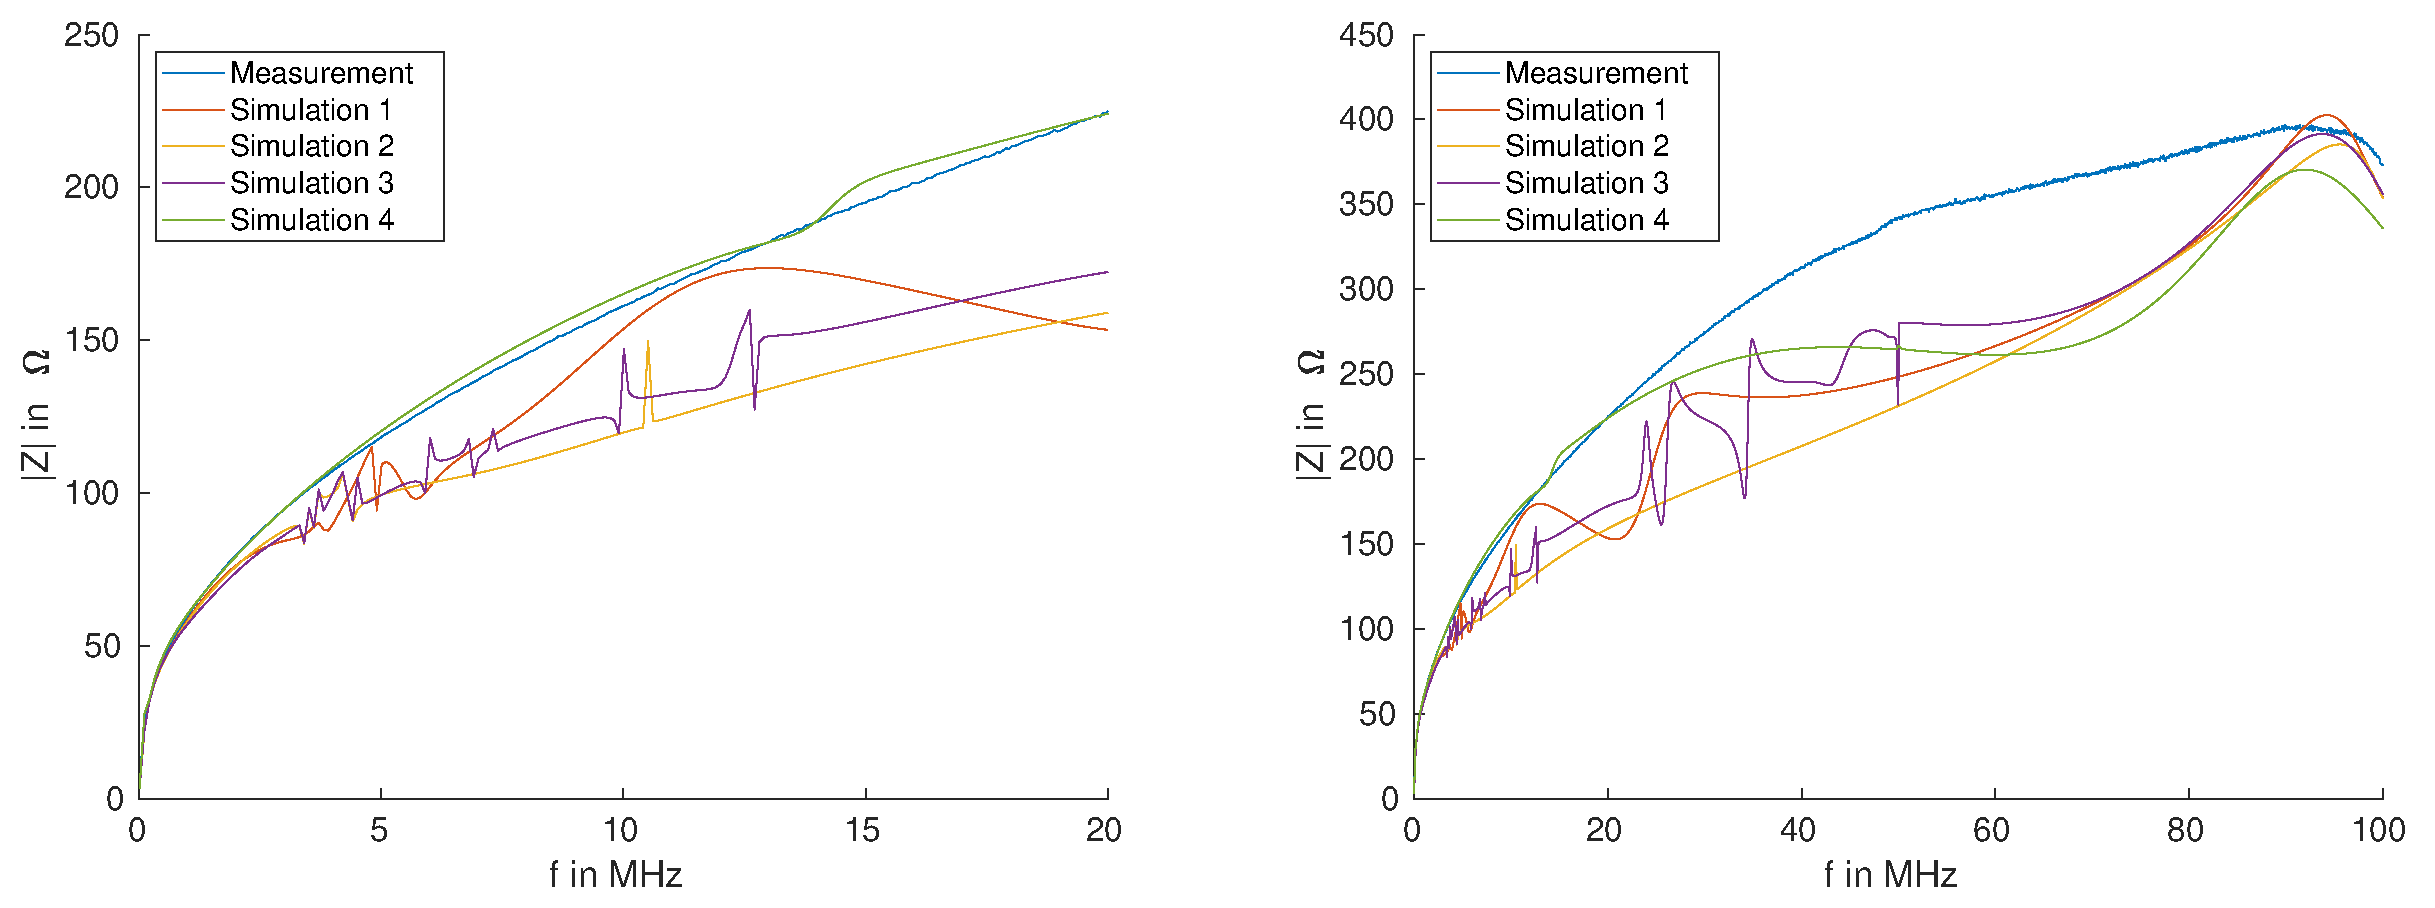
\includegraphics[width=0.95\textwidth]{Zges_RK_SimMeas}
\end{figure}
\end{frame}



\begin{frame}\frametitle{Gegen\"uberstellung der Simulations- und Messergebnisse (mit einem Kurzschluss)}
\vspace{-1em}
\begin{figure}[h]
	\centering
	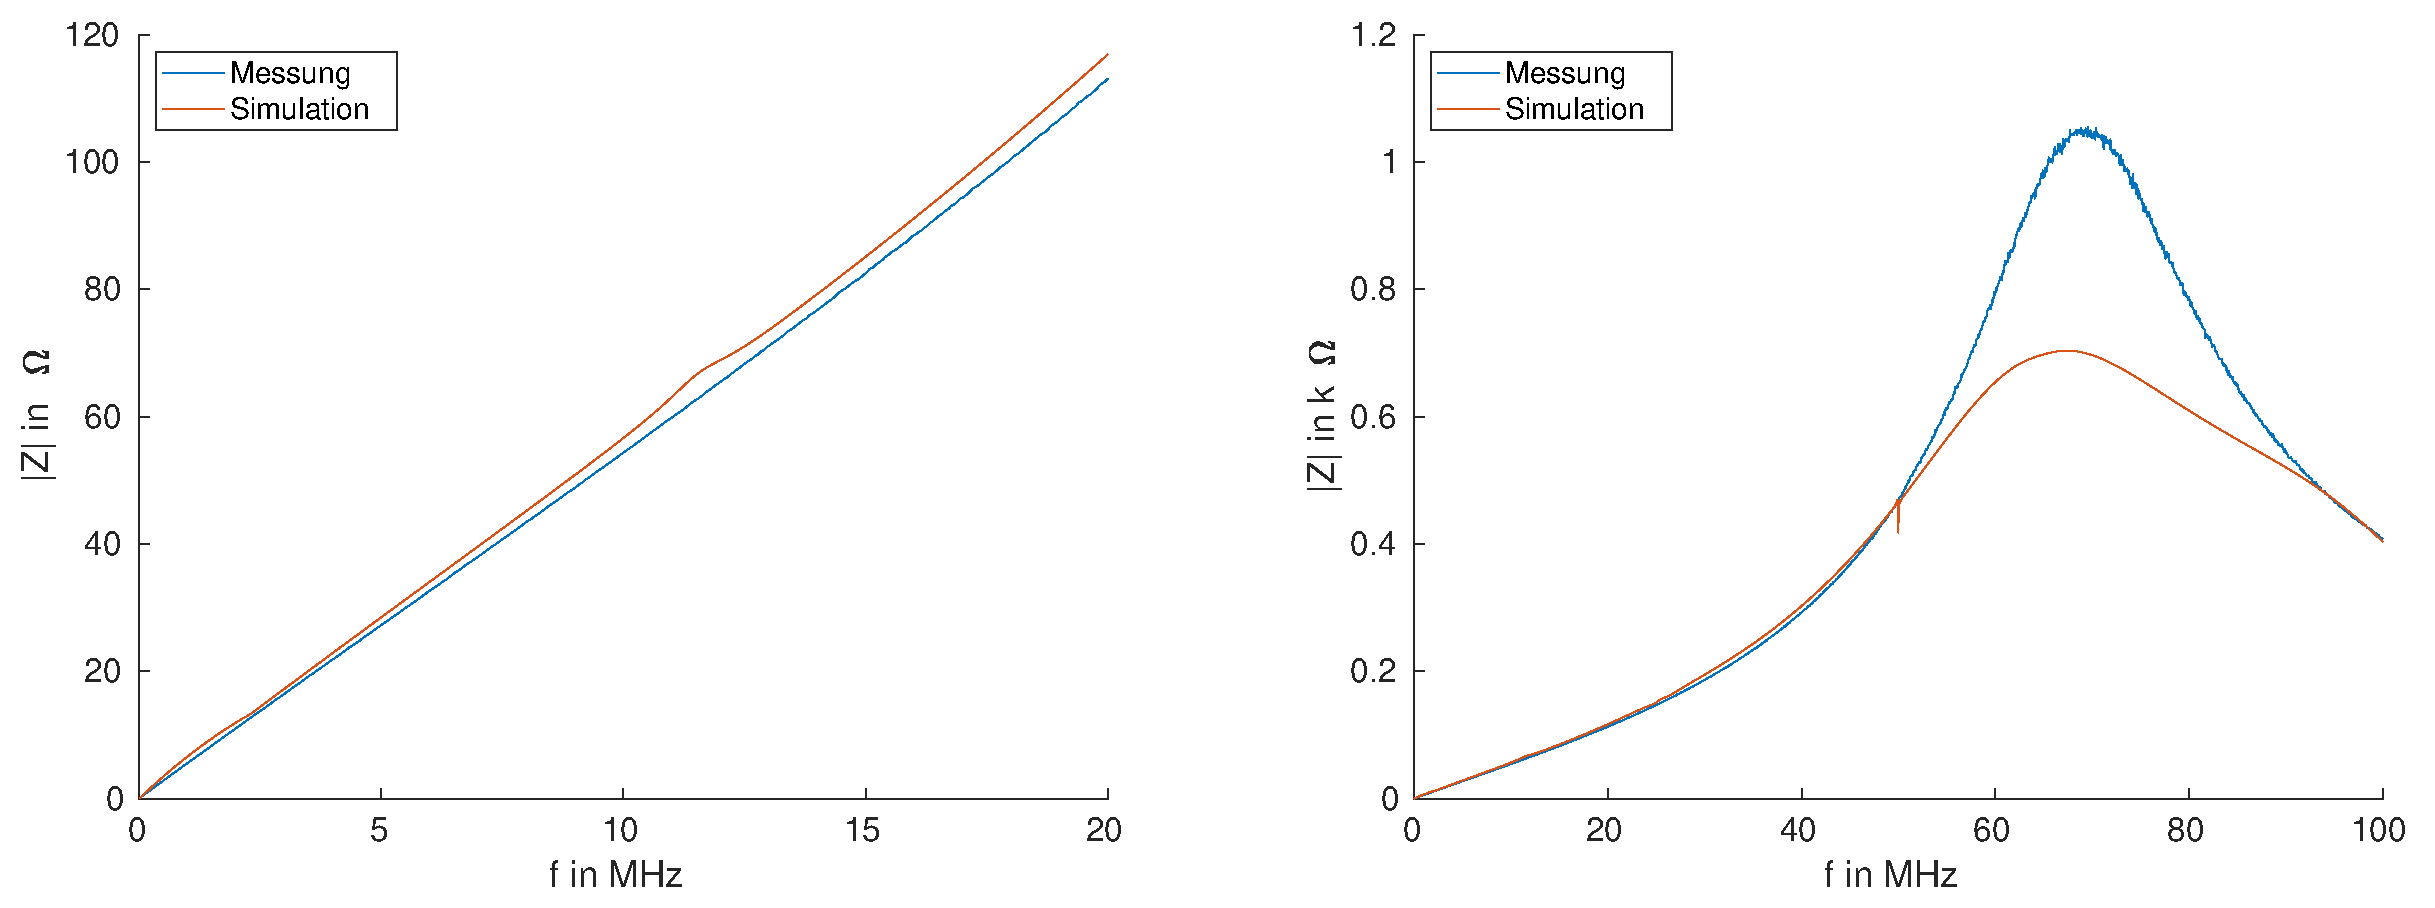
\includegraphics[width=0.95\textwidth]{Z_ges_1KS_SimMeas}
\end{figure}
\end{frame}



%%%%%%%%%%%%%%%%%%%%%%%%%%%%%%%%%%%%%%%%%%%%%%%%%%%%%%%%%%%%%%%%%%%%%%%%%%%%%%%%%%%%%%%%%%%%%%%%%%%%%%%%%%%%%%%%%%%%%%%%%%%%%%%%%%%
%%%%%%%%%%%%%%  TEIL3: Rainer %%%%%%%%%%%%%%%%%%%%%%%%%%%%%%%%%%%%%%%%%%%%%%%%%%%%%%%%%%%%%%%%%%%%%%%%%%%%%%%%%%%%%%%%%%%%%%%%%%%%%


\begin{frame}\frametitle{Anzahl der Kurzschl\"usse}
\vspace{-1em}
\begin{figure}[h]
	\centering
	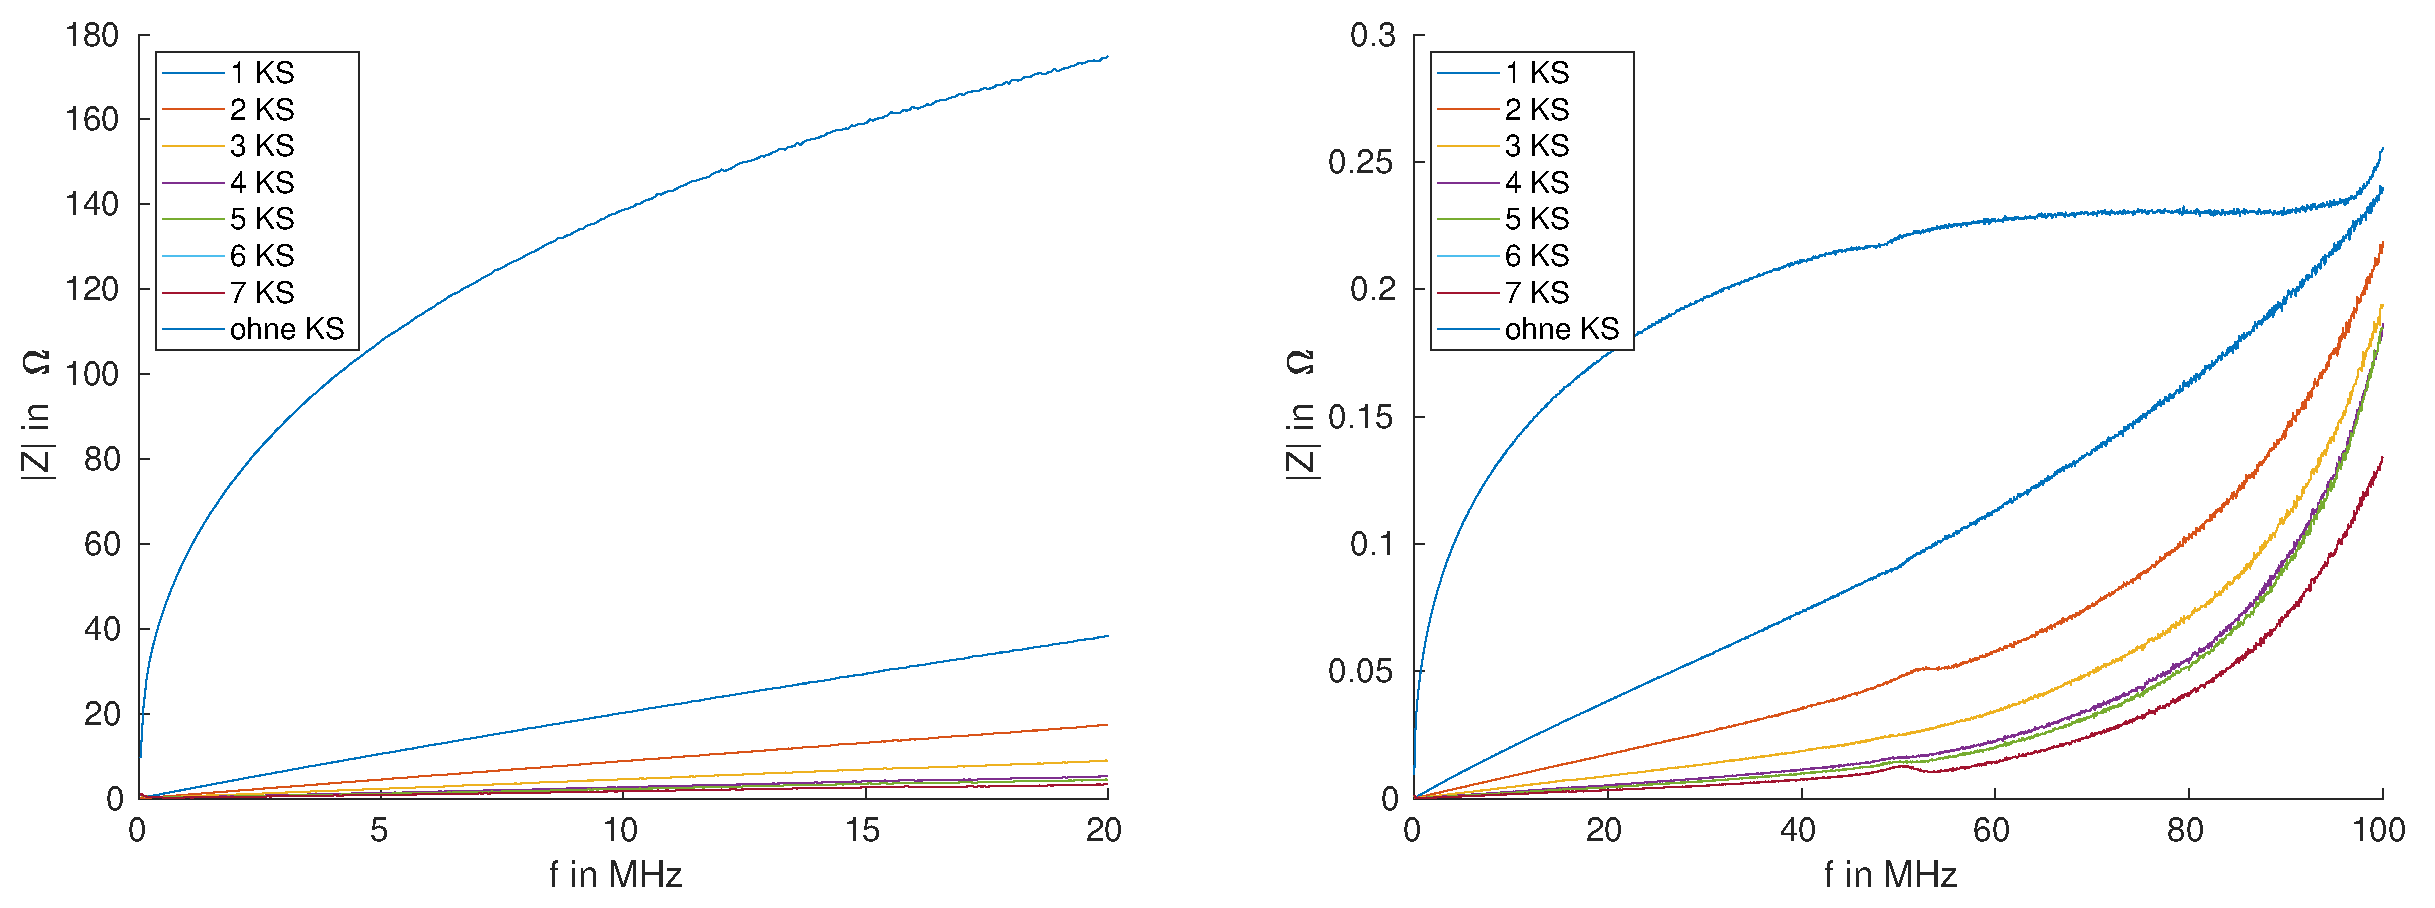
\includegraphics[width=0.95\textwidth]{impedance_numberKS_ringcore}
\end{figure}
\end{frame}


\begin{frame}\frametitle{Anzahl der Kurzschl\"usse}
 \vspace{-1em}
\begin{figure}[h]
	\centering
	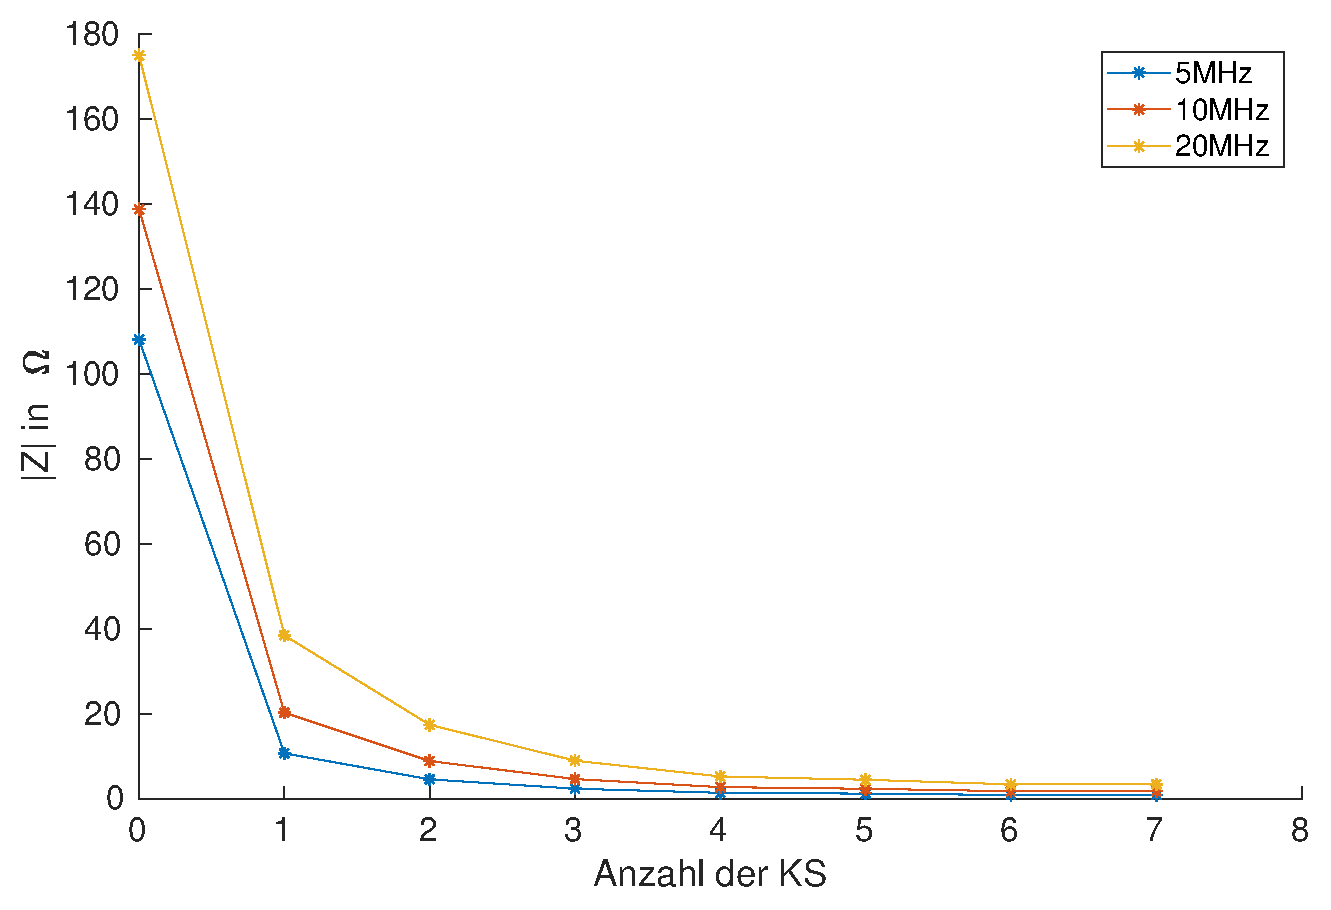
\includegraphics[width=0.65\textwidth]{RK_Impedanz_numberKS_frequenz}
\end{figure}
\end{frame}


\begin{frame}\frametitle{Feldverteilung f\"ur verschiedene Anzahlen an Kurzschl\"ussen}
\vspace{-2.75em}
\begin{figure}[htb]
% 	\centering
	\flushleft
	\subfloat[kein KS]{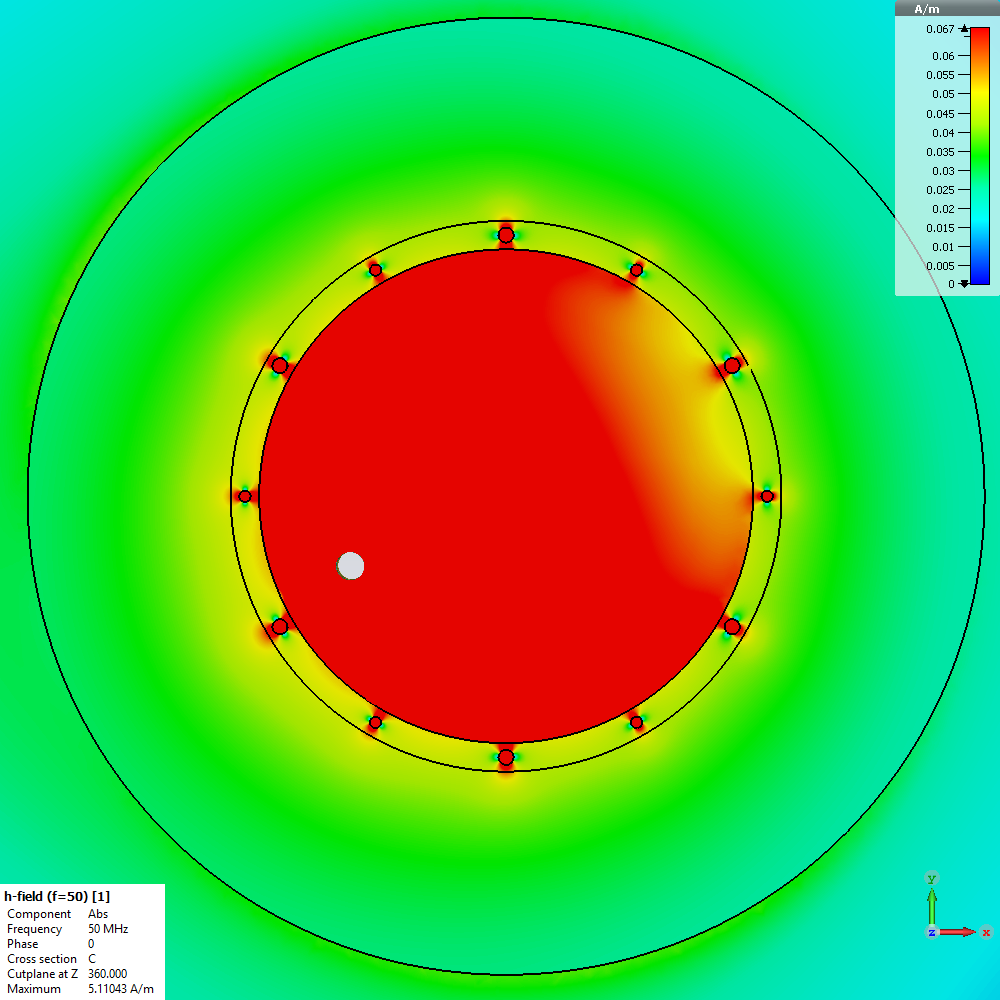
\includegraphics[height=0.23\textwidth]{Feldbilder/0KS}}
	\hspace{0.0312\textwidth}
	\subfloat[1 KS]{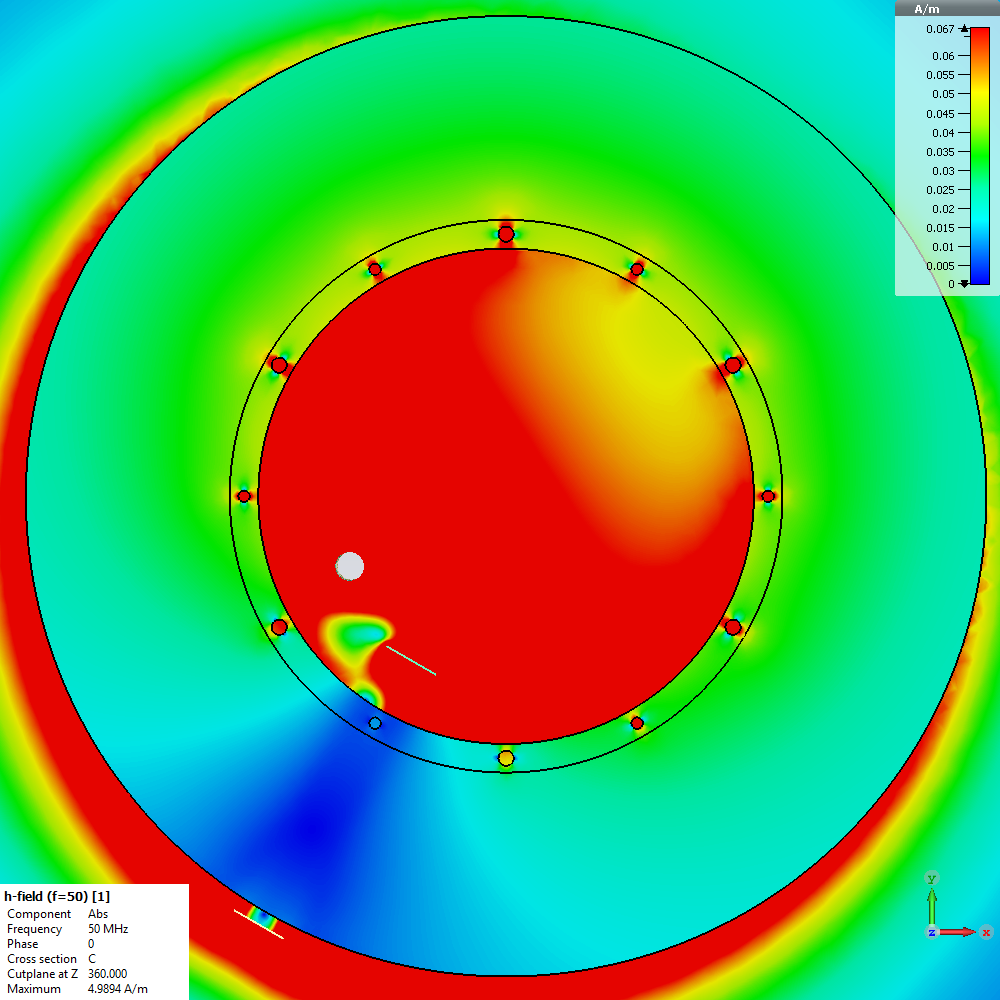
\includegraphics[height=0.23\textwidth]{Feldbilder/1KS}}
	\hspace{0.0312\textwidth}
	\subfloat[2 KS]{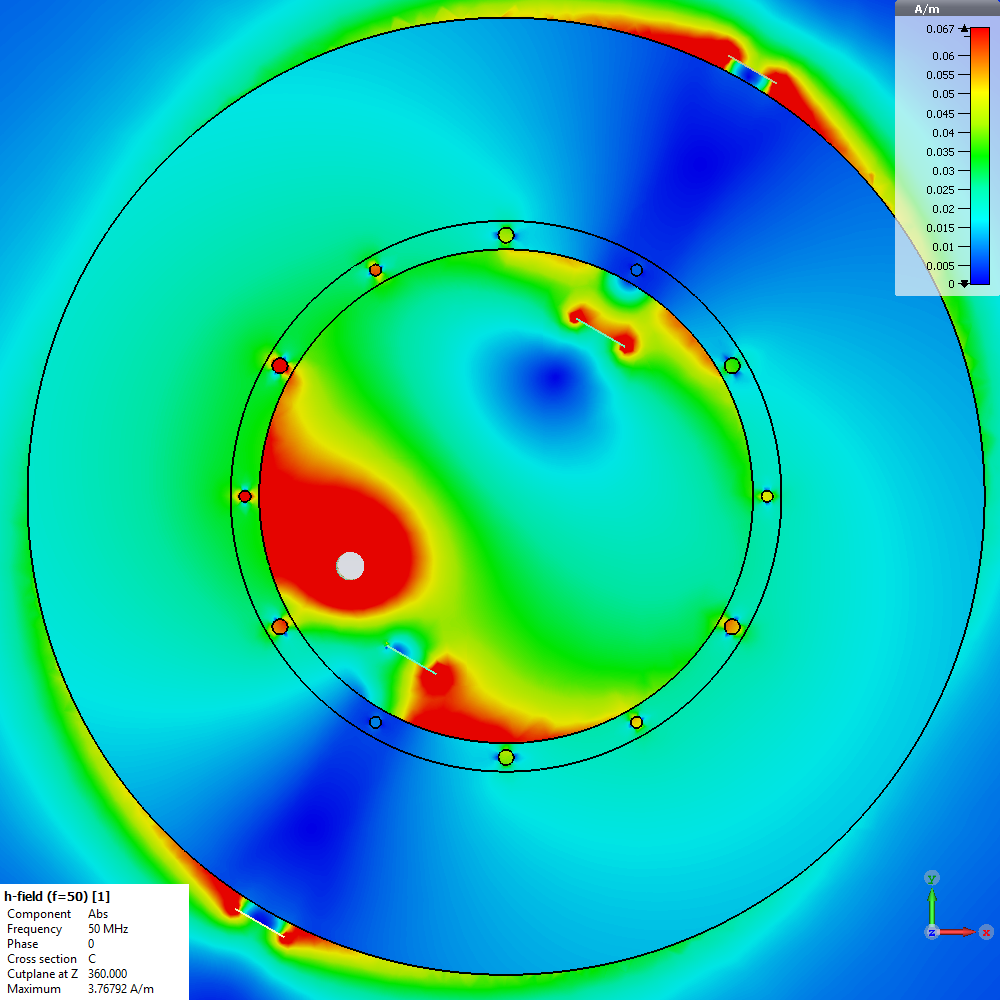
\includegraphics[height=0.23\textwidth]{Feldbilder/2KS}}
	\\ \vspace{-1em}
	\subfloat[3 KS]{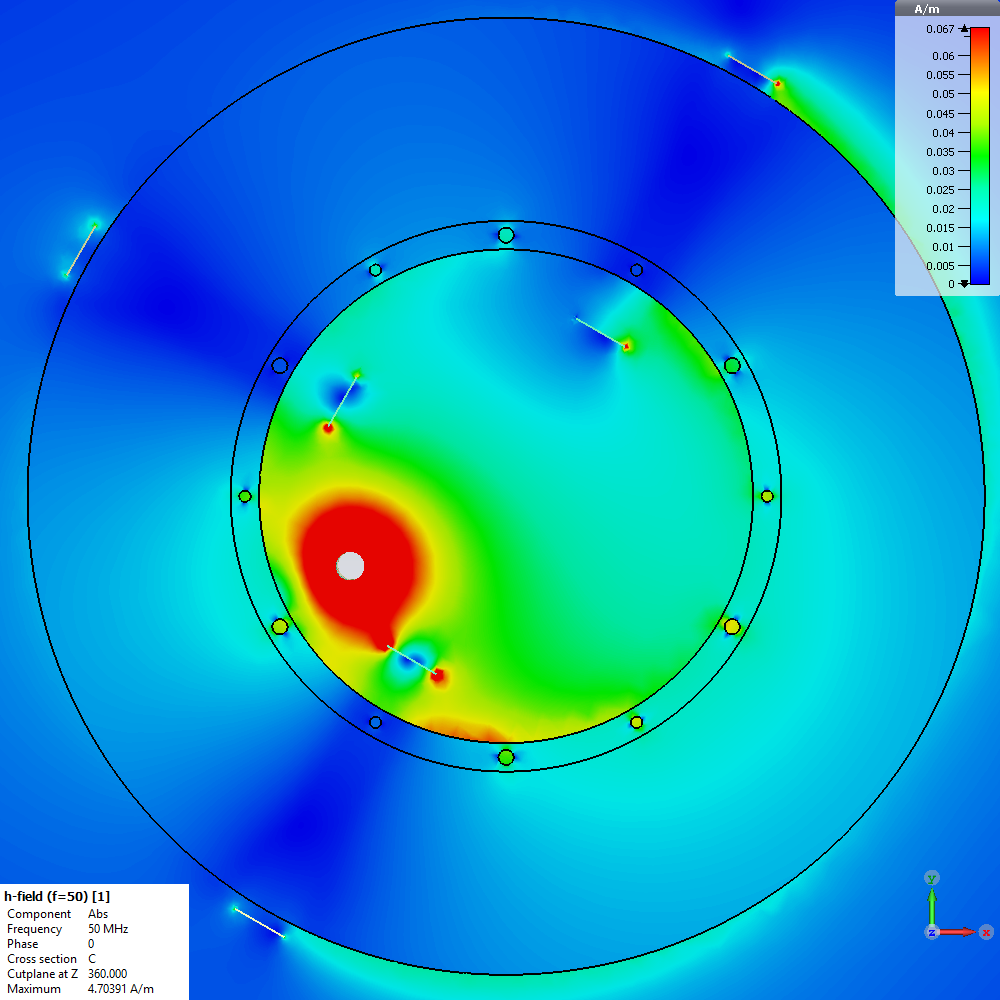
\includegraphics[height=0.23\textwidth]{Feldbilder/3KS}}
% 	\subfloat[4 KS]{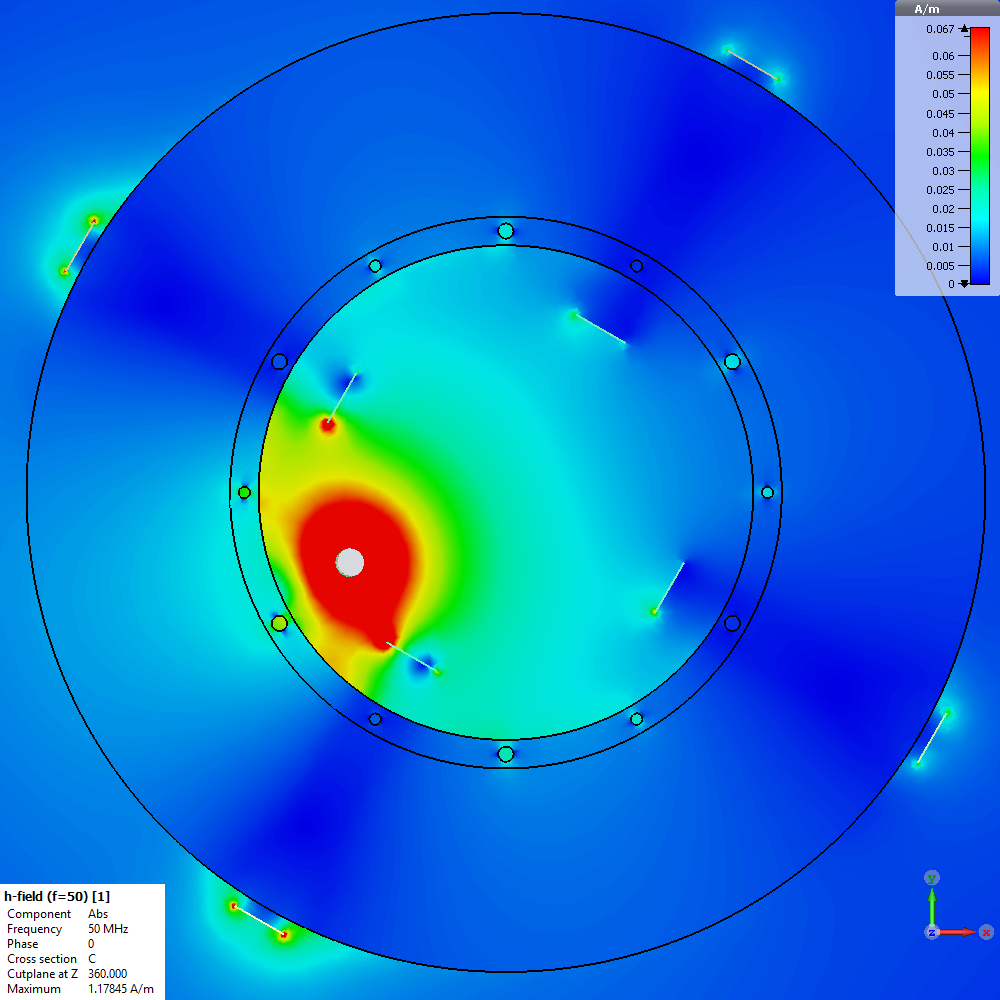
\includegraphics[height=0.23\textwidth]{Feldbilder/4KS}}
	\hspace{0.0312\textwidth}
	\subfloat[5 KS]{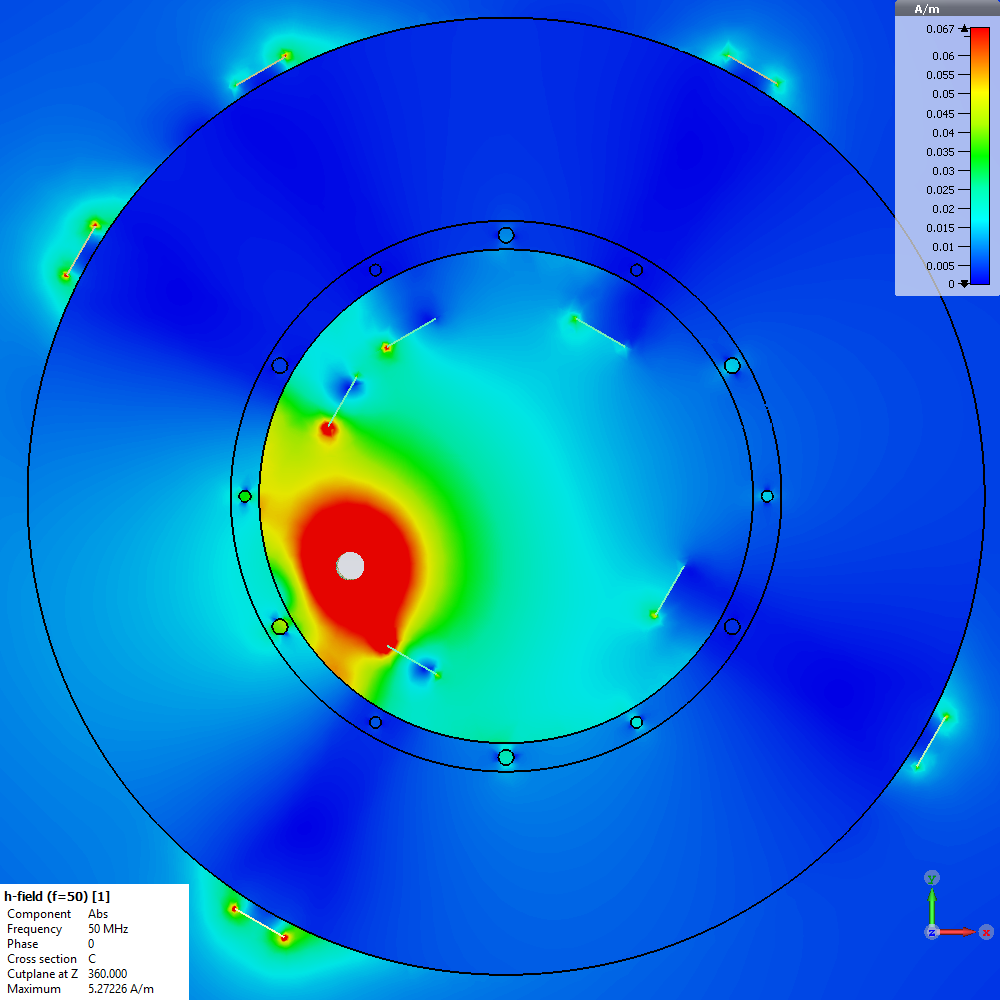
\includegraphics[height=0.23\textwidth]{Feldbilder/5KS}}
% 	\subfloat[6 KS]{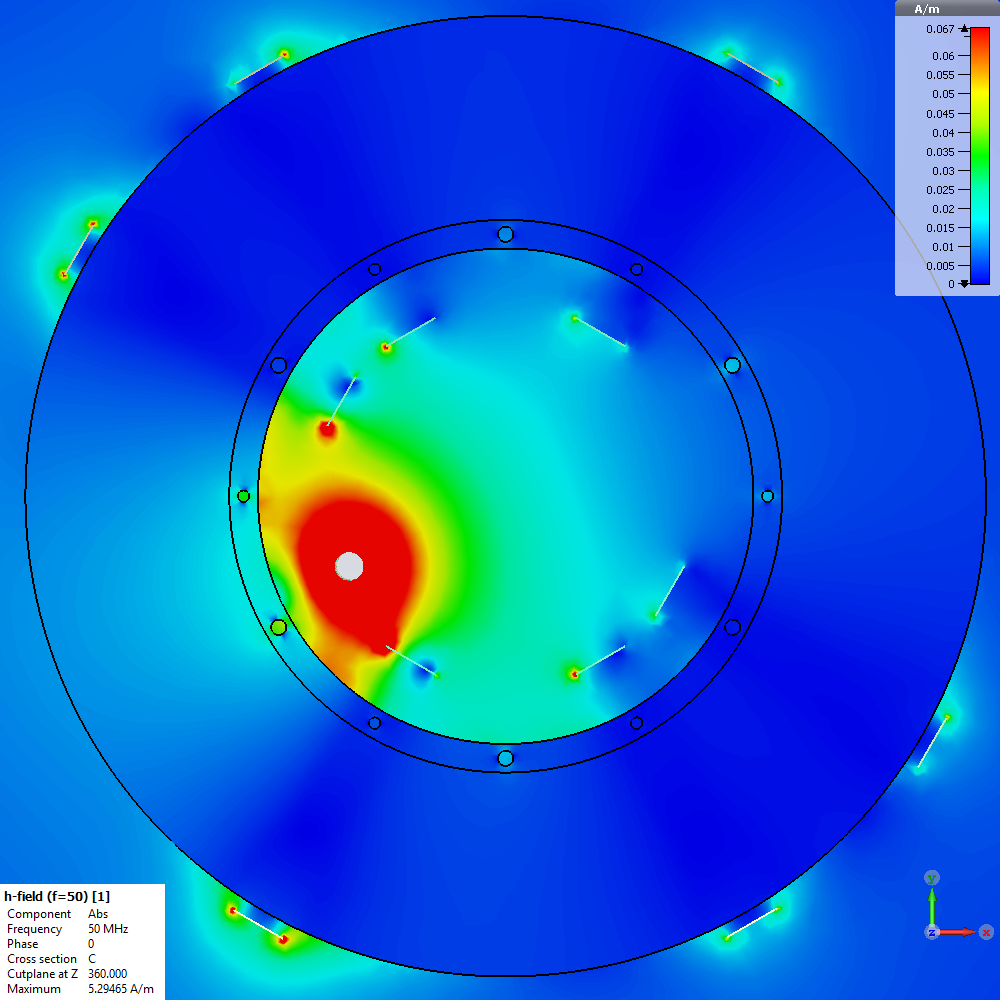
\includegraphics[height=0.23\textwidth]{Feldbilder/6KS}}
	\hspace{0.0312\textwidth}
	\subfloat[7 KS]{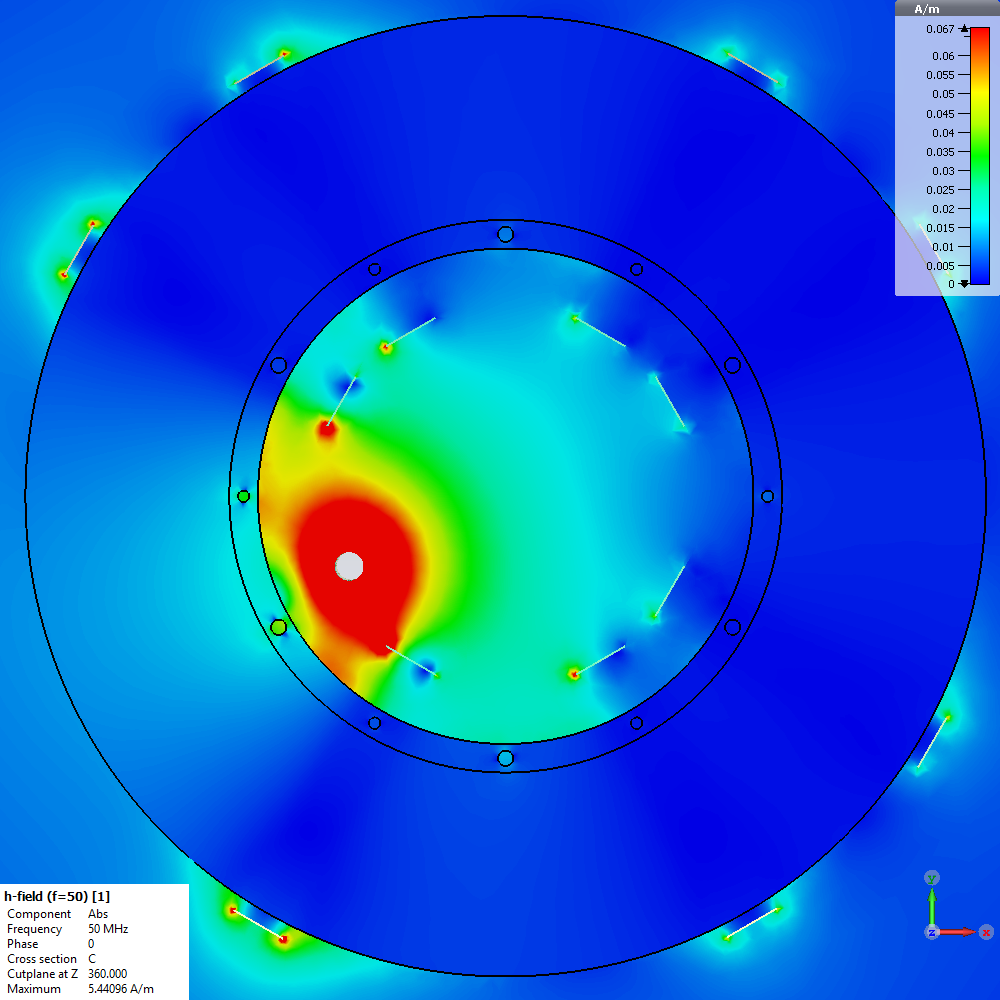
\includegraphics[height=0.23\textwidth]{Feldbilder/7KS}}
\end{figure}
\vspace{-0.605\textwidth}
\begin{figure}[t]
	\flushright
	\subfloat{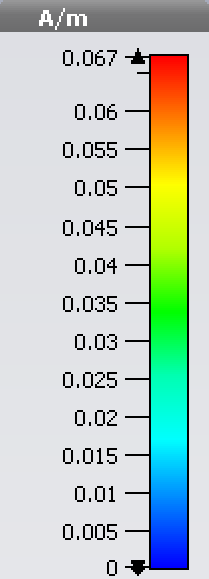
\includegraphics[width=0.183\textwidth]{Feldbilder/legend}}
\end{figure}

\end{frame}


\begin{frame}\frametitle{Breite der Kurzschlüsse}
\vspace{-1em}
\begin{figure}[h]
	\centering
	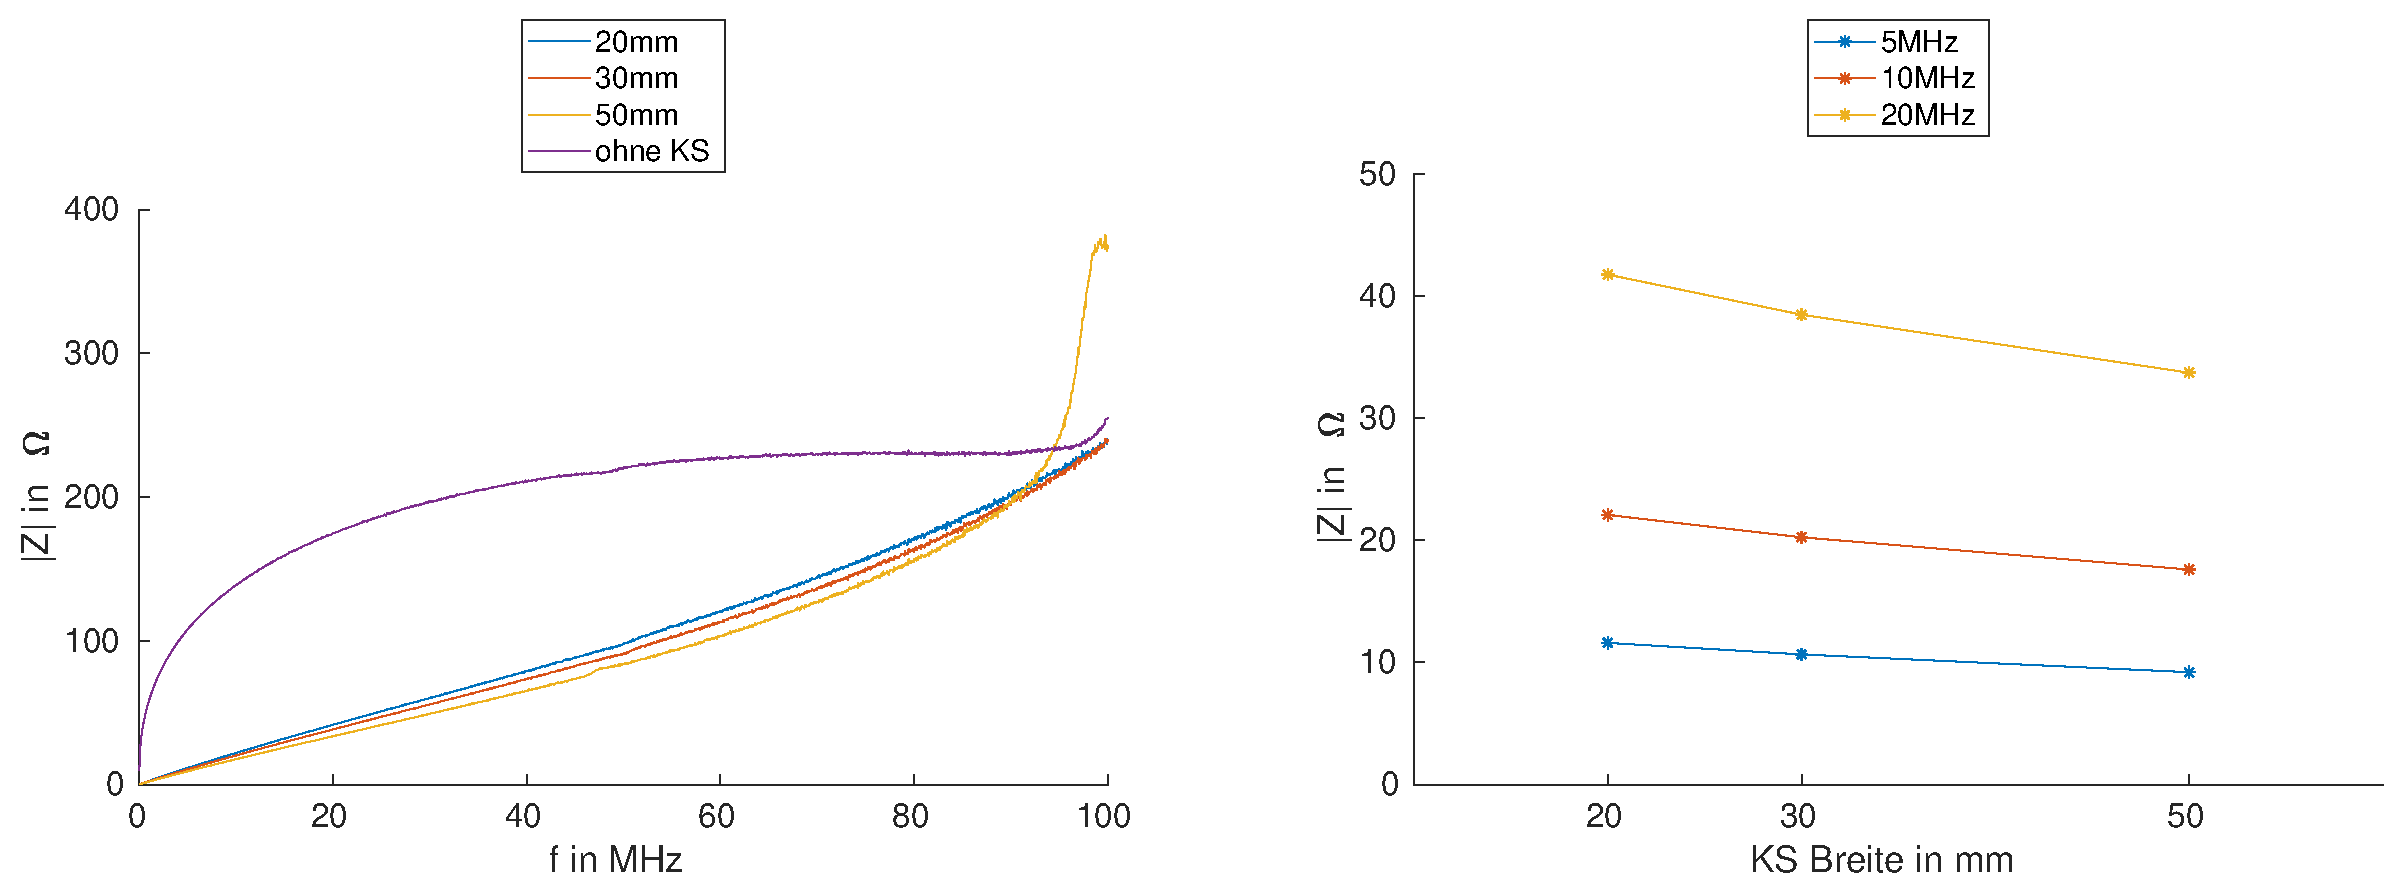
\includegraphics[width=0.95\textwidth]{Z_ges_width_frequency_SimMeas}
\end{figure}
\end{frame}


% \begin{frame}\frametitle{Breite der Kurzschlüsse}
% \vspace{-1em}
% \begin{figure}[h]
% 	\centering
% 	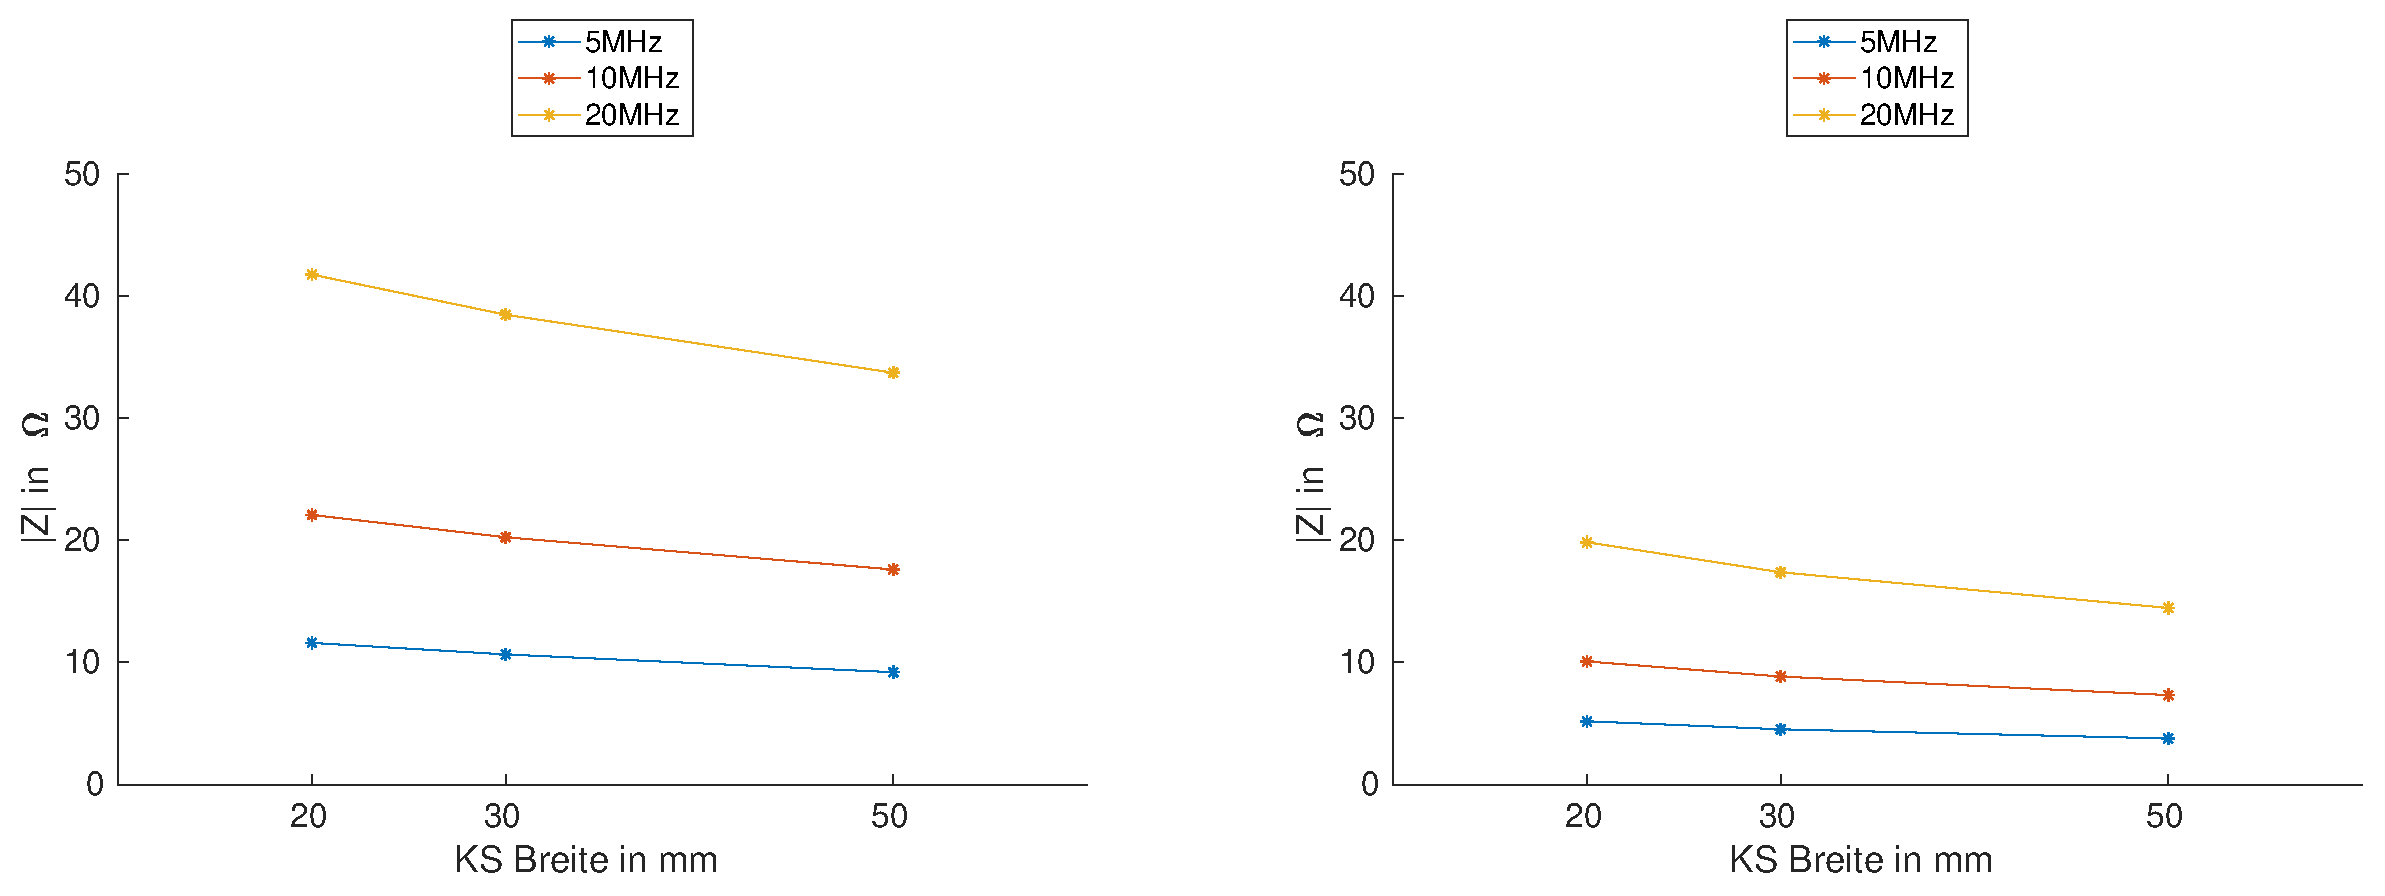
\includegraphics[width=0.95\textwidth]{RK_Impedanz_width_frequenz}
% \end{figure}
% \end{frame}

\begin{frame}\frametitle{Länge der Kurzschlüsse}
\vspace{-1em}
\begin{figure}[h]
	\centering
	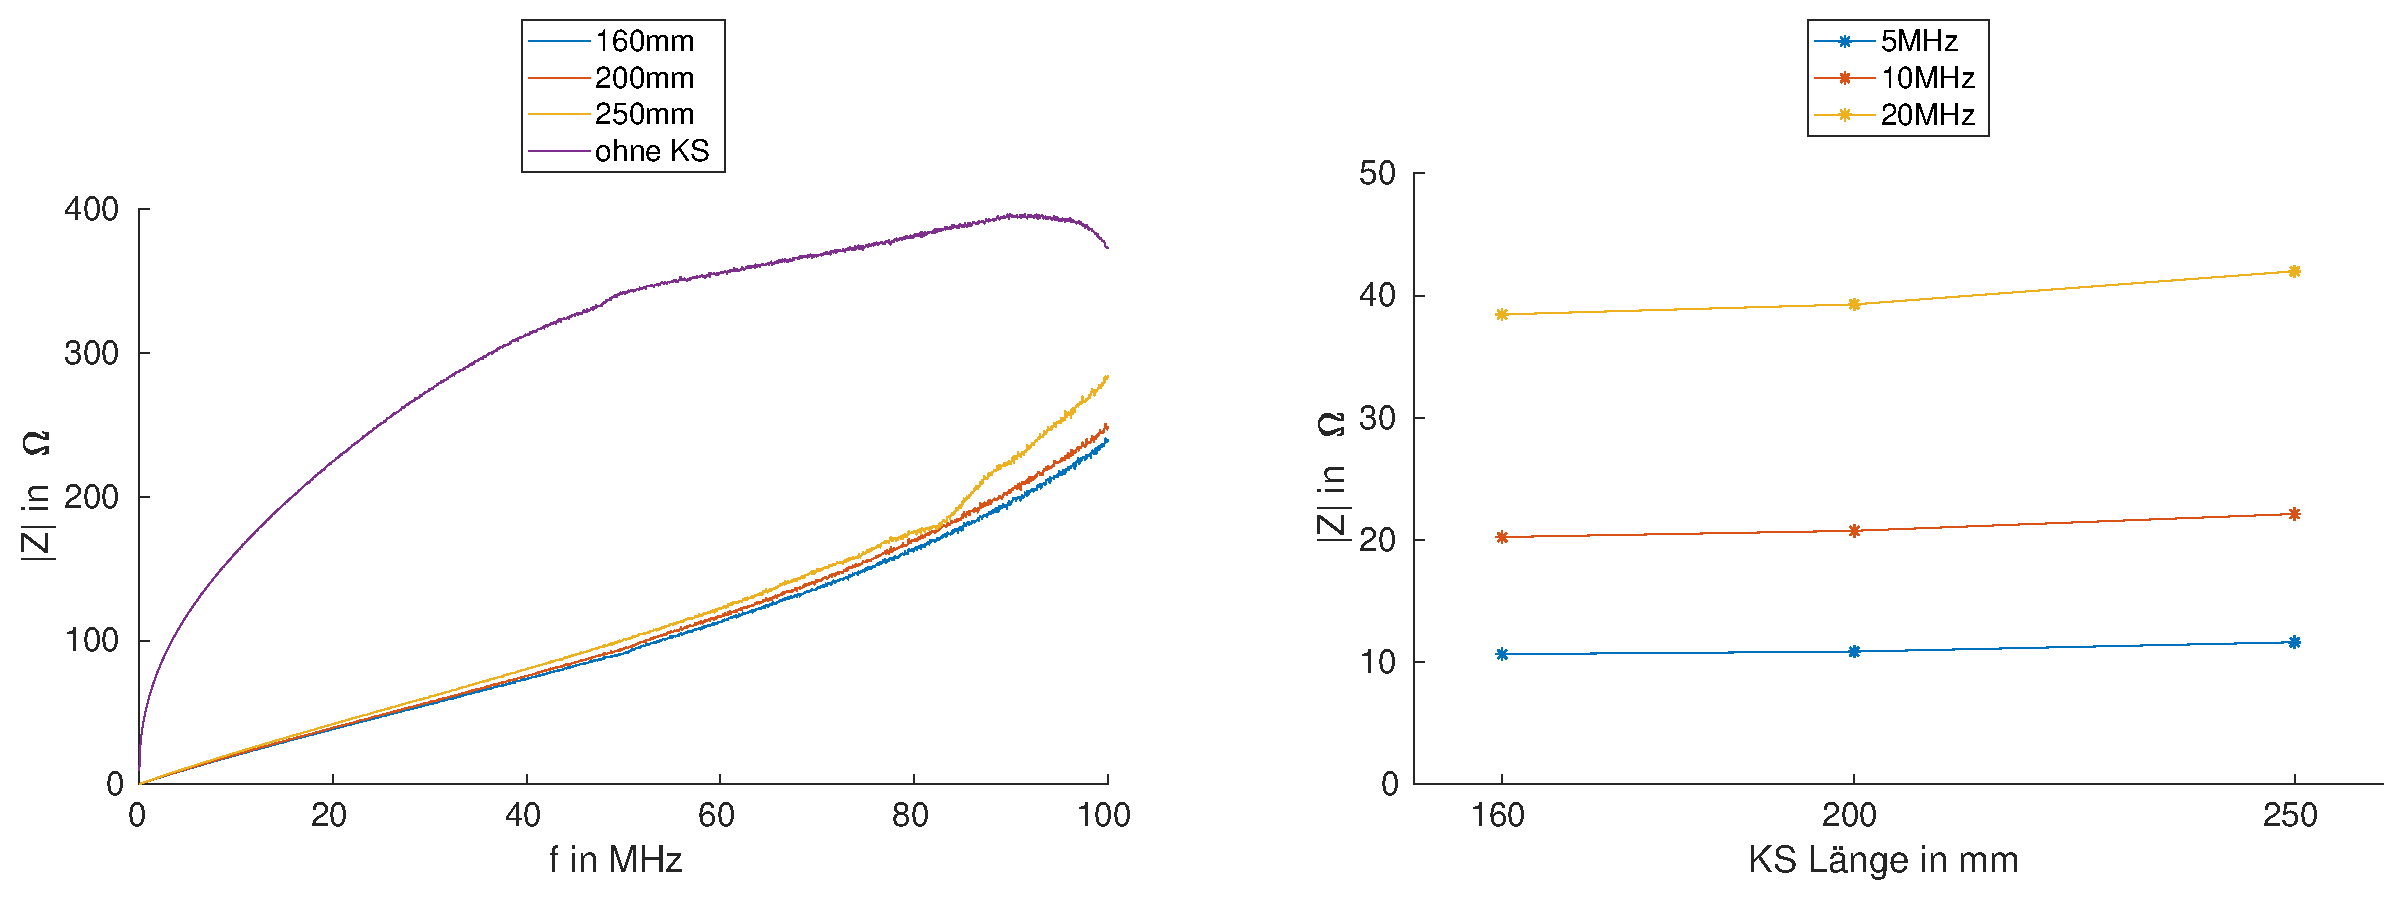
\includegraphics[width=0.95\textwidth]{Z_ges_length_frequency_SimMeas}
\end{figure}
\end{frame}


% \begin{frame}\frametitle{Länge der Kurzschlüsse}
% \vspace{-1em}
% \begin{figure}[h]
% 	\centering
% 	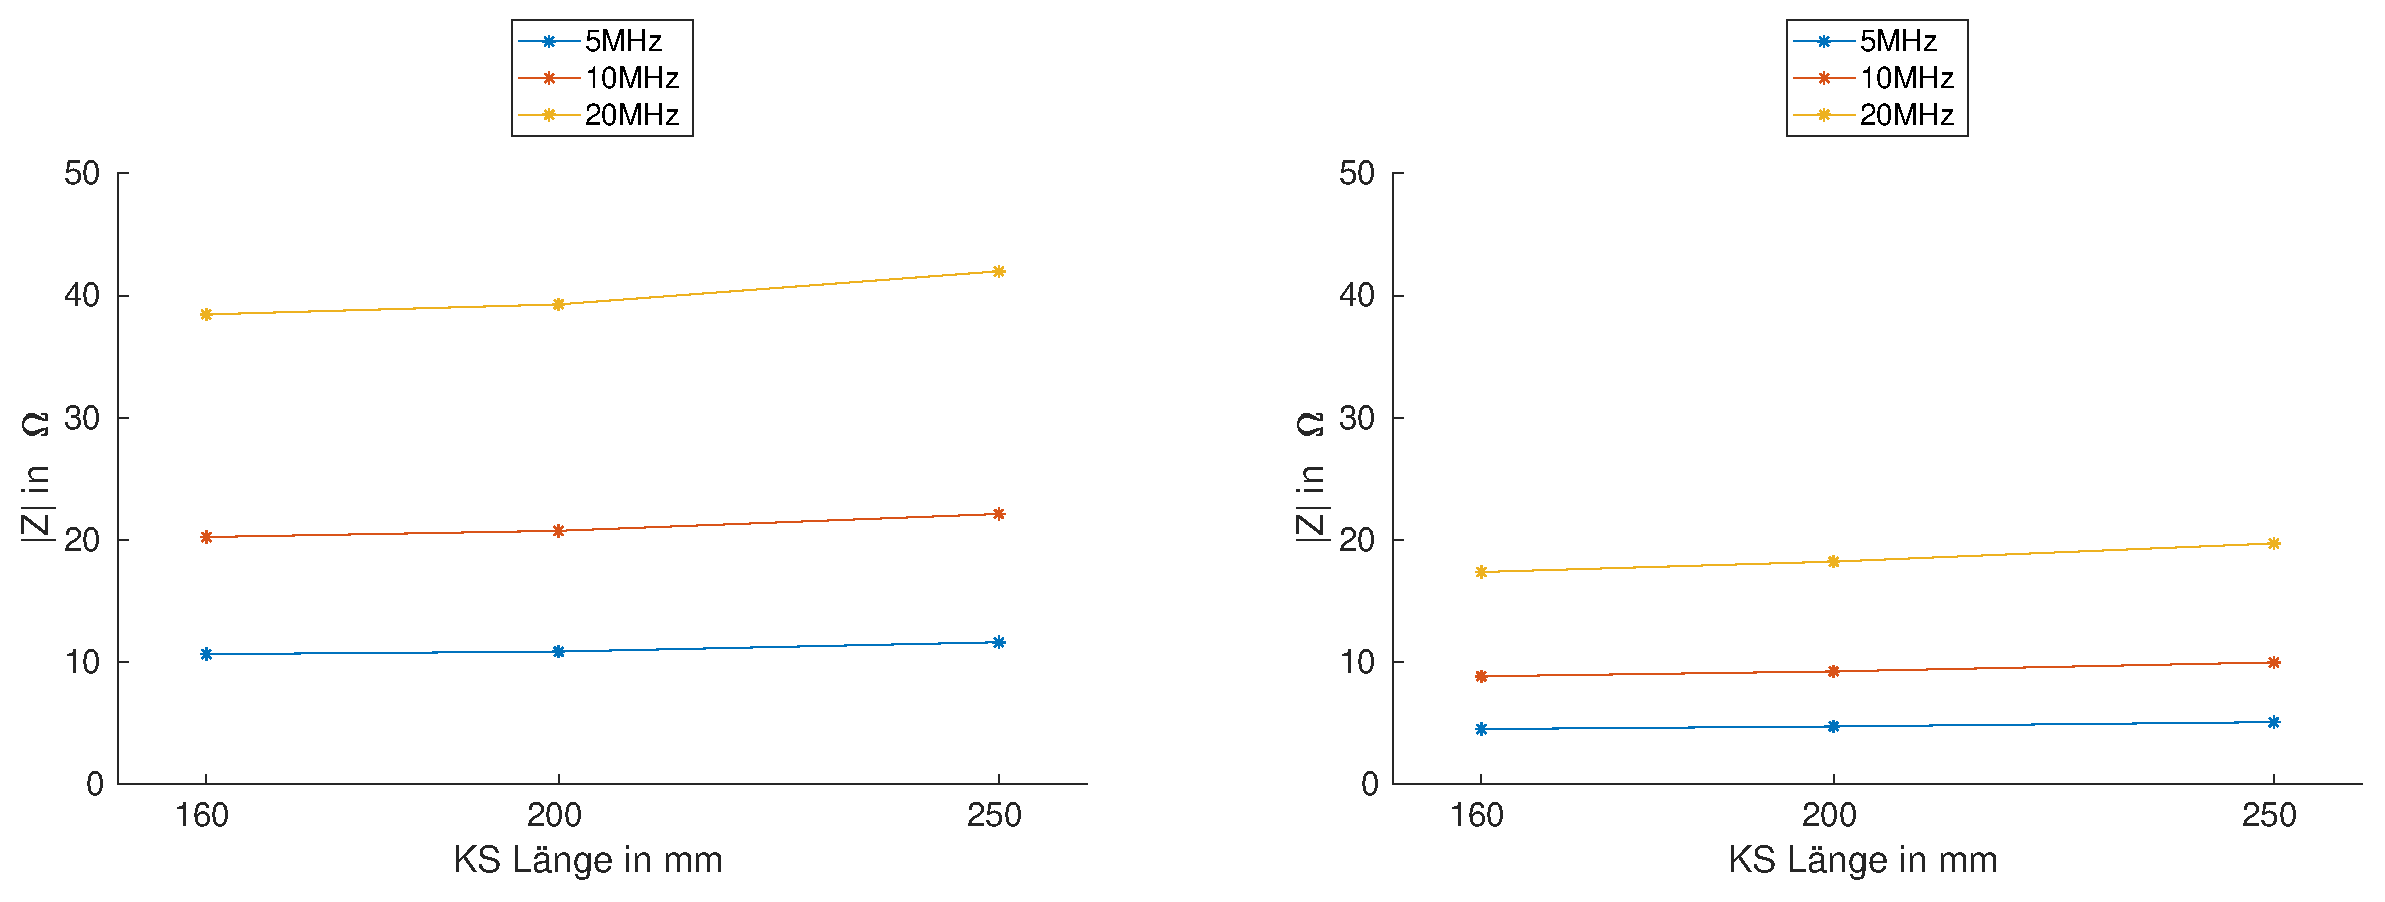
\includegraphics[width=0.95\textwidth]{RK_Impedanz_length_frequenz}
% \end{figure}
% \end{frame}



\begin{frame}\frametitle{Dicke der Kurzschlüsse}
\vspace{-1em}
\begin{figure}[h]
	\centering
	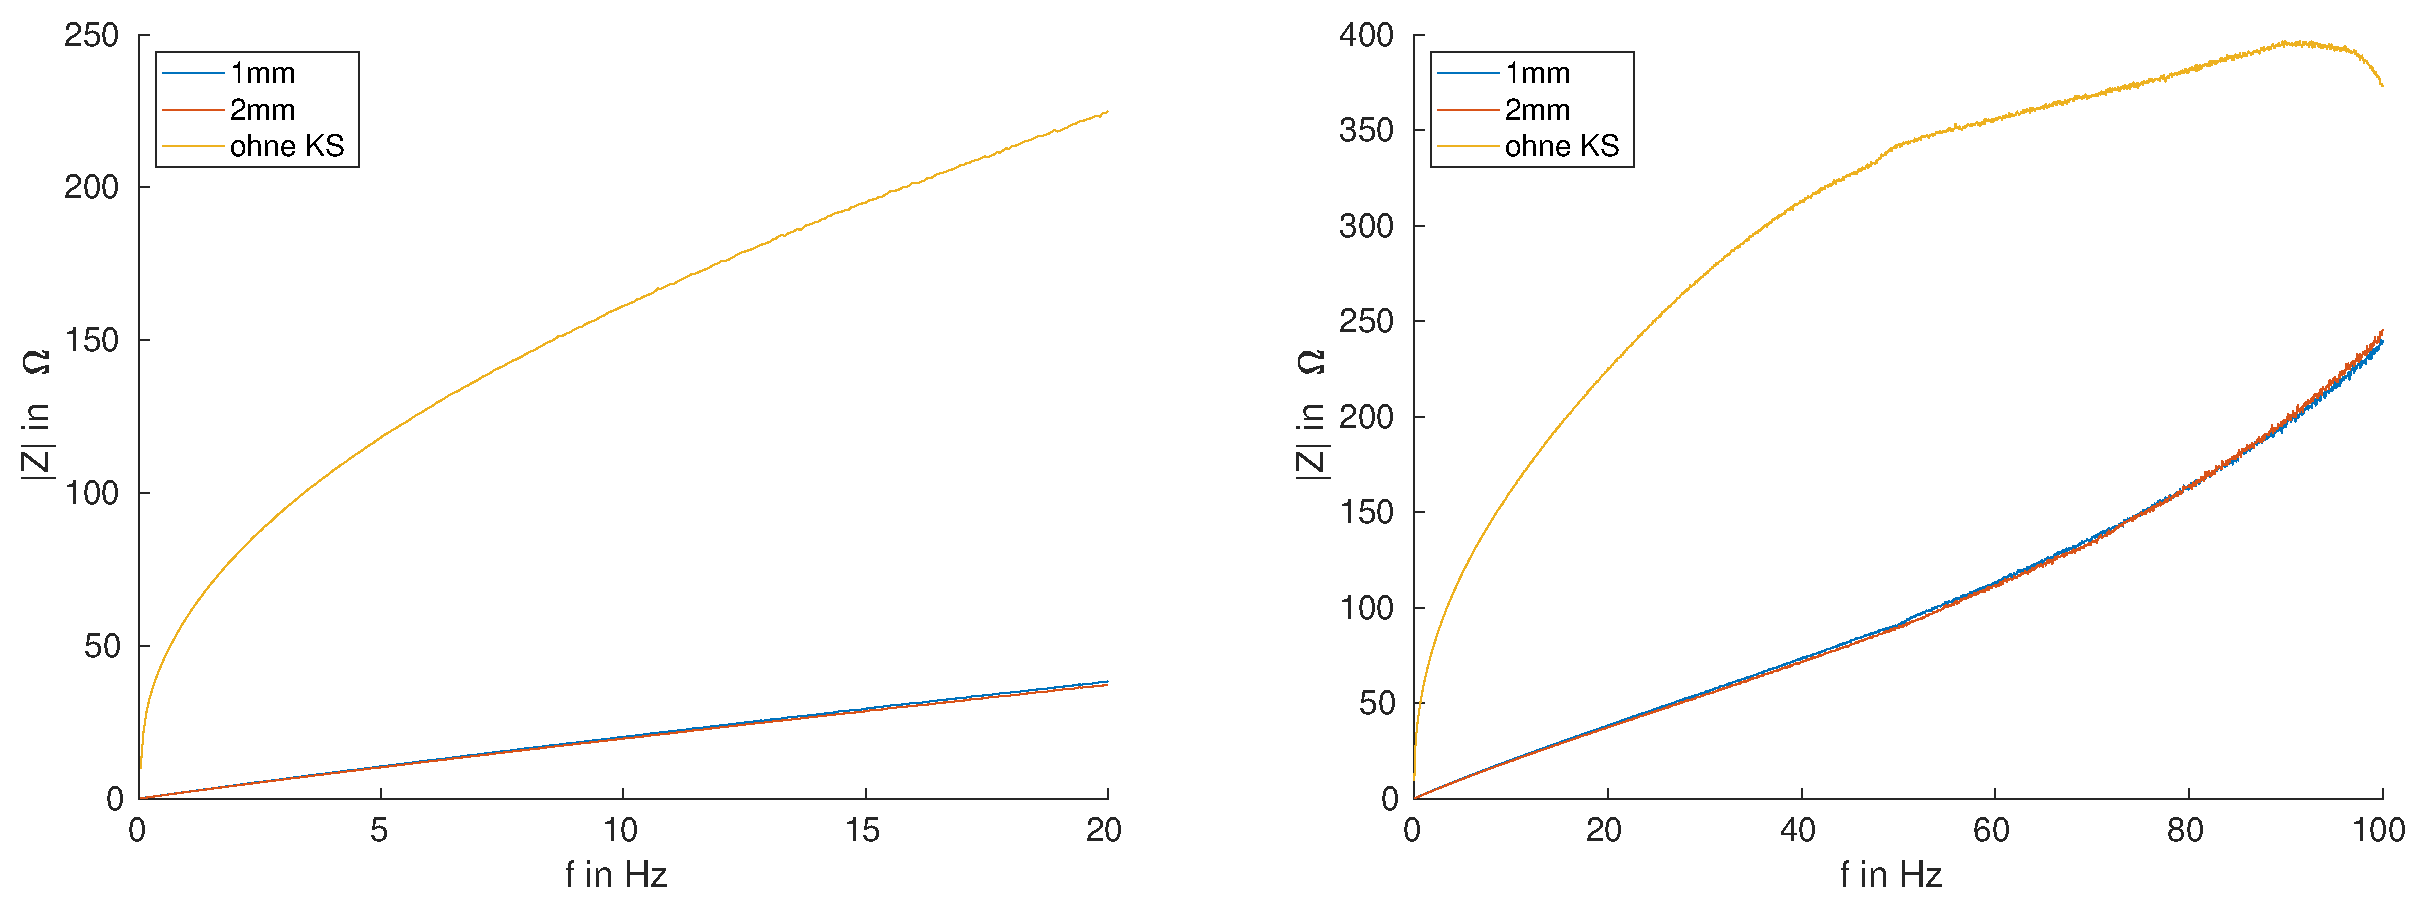
\includegraphics[width=0.95\textwidth]{Z_RK_thick_1KS}
\end{figure}
\end{frame}



\begin{frame}\frametitle{Einfluss im Leerlauf befindlicher Schienen auf die Ringkernimpedanz}
\vspace{-1em}
\begin{figure}[h]
	\centering
	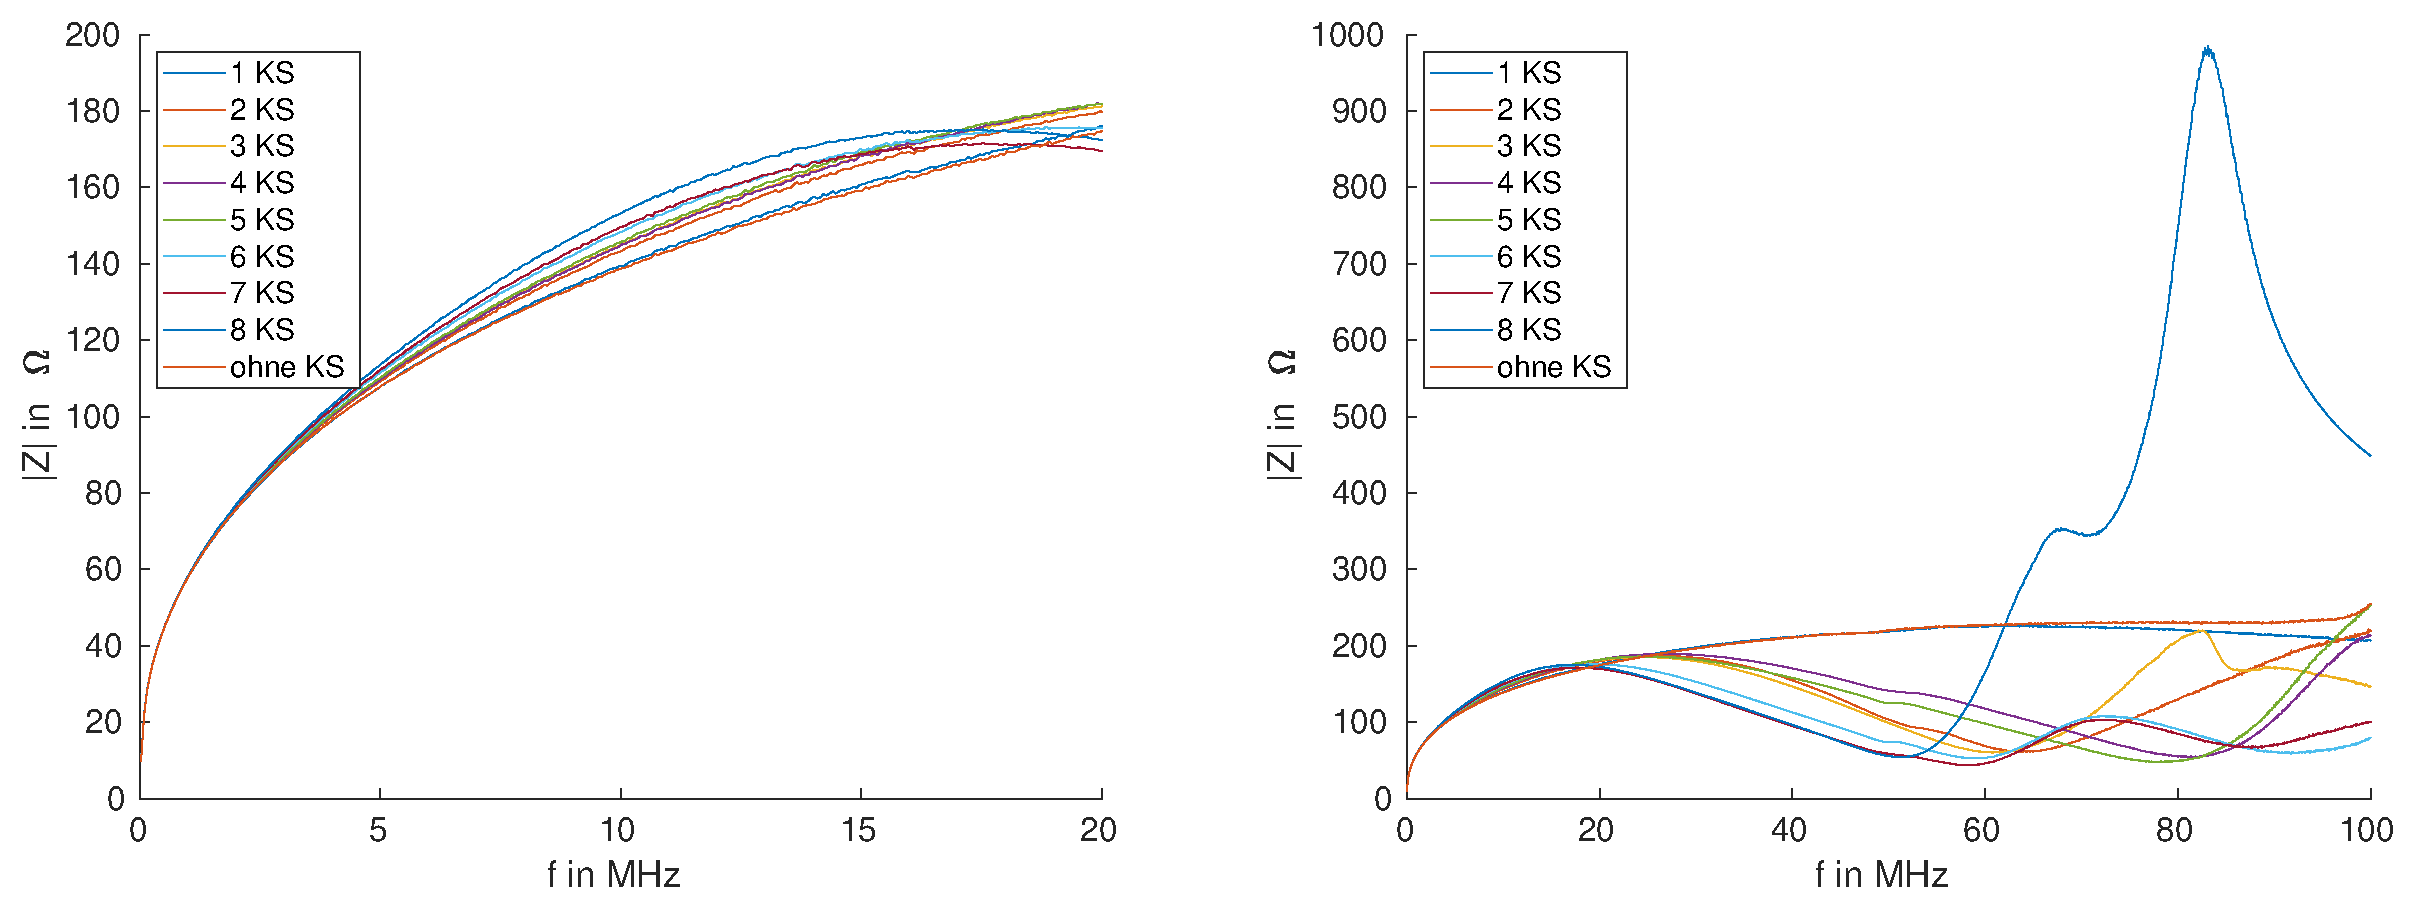
\includegraphics[width=0.95\textwidth]{Z_RK_numKS_open}
\end{figure}
\end{frame}


\begin{frame}\frametitle{\"Ubertragung in die Kavit\"at}
\begin{minipage}[t]{0.33\textwidth}
	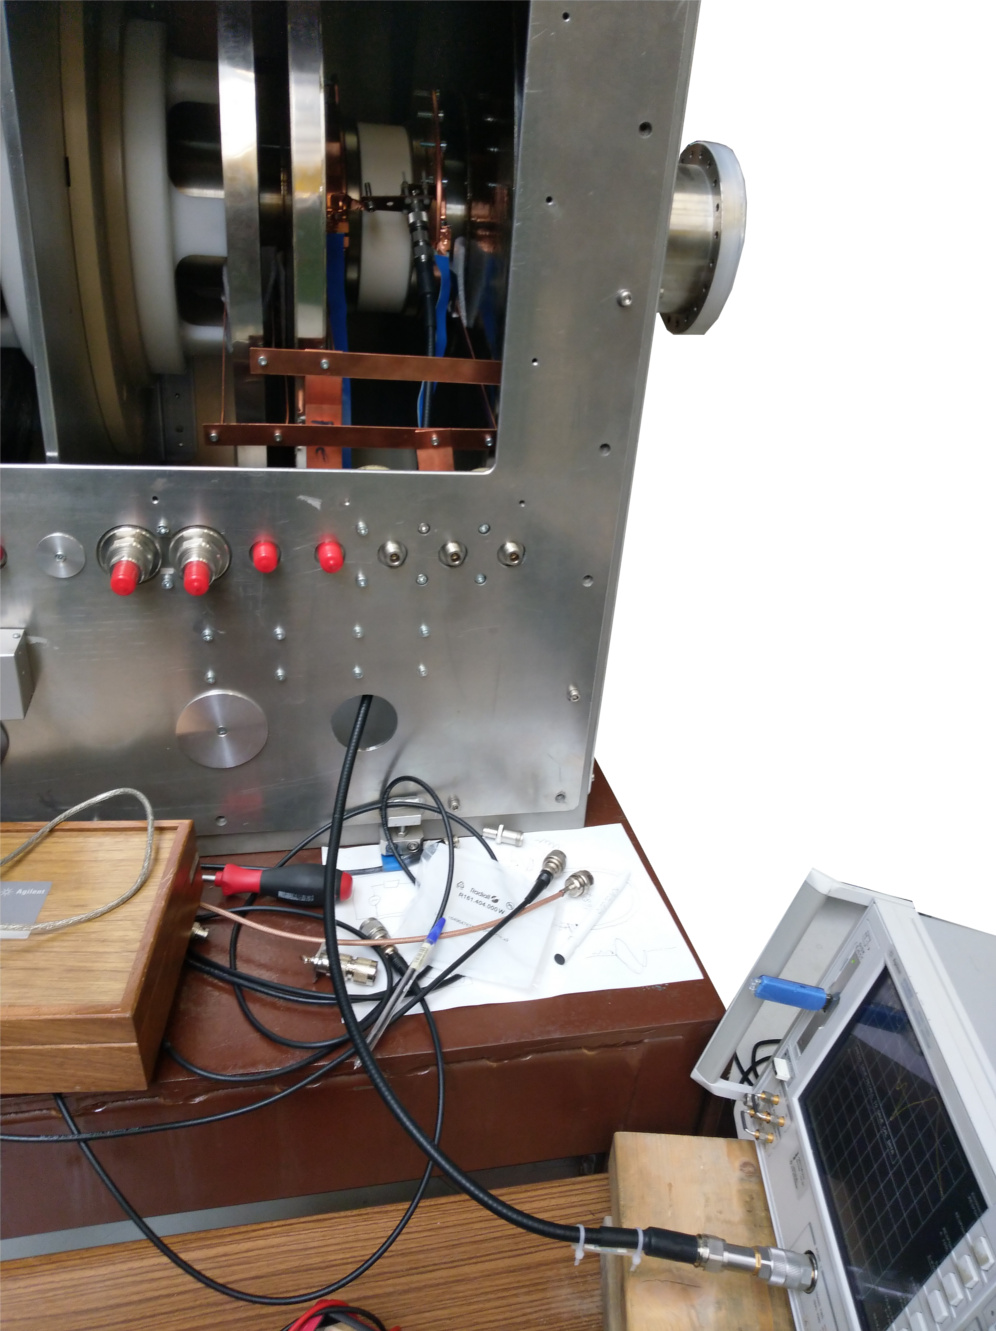
\includegraphics[width=\textwidth]{Messung_Kavitaet_NA_crop}
\end{minipage}
\begin{minipage}[t]{0.6\textwidth}
	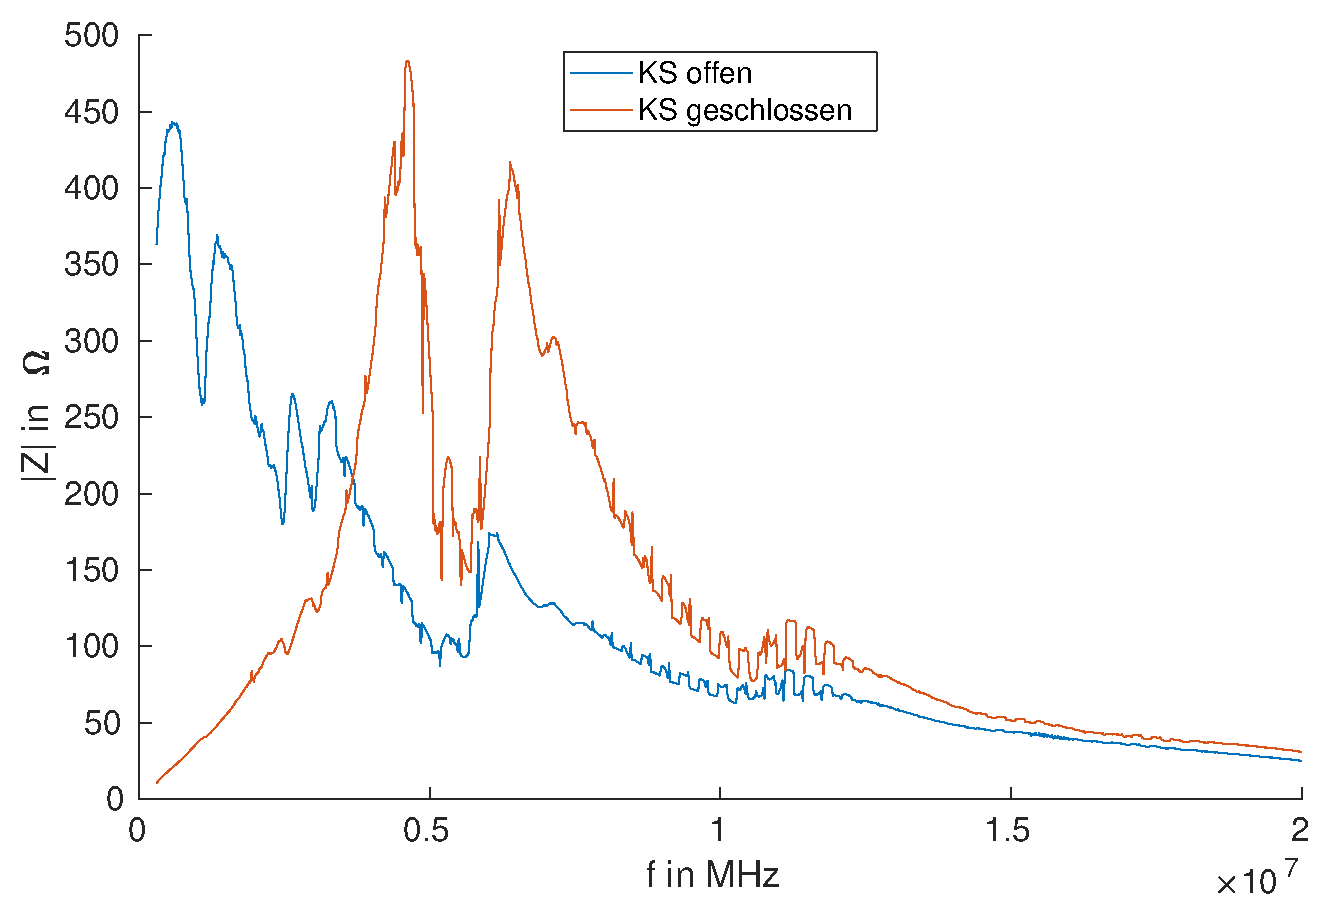
\includegraphics[width=\textwidth]{Z_ges_cavity}
\end{minipage}
\end{frame}

\begin{frame}\frametitle{Zusammenfassung}
\begin{itemize}
	\item Messung Testbox
	\item Modifikation 
	\item Reproduzierbare Messungen
	\item Simulation
	\item Ergebnisse quantifiziert, evaluiert
\end{itemize}
\end{frame}


\begin{frame}\frametitle{Fazit und Ausblick}
\begin{itemize}
	\item Reduktion ein Kurzschluss: \textbf{80\,\%}
	\item Reduktion sieben Kurzschl\"usse:  \textbf{>\,98\,\%}
	\item Geringer Einfluss restlicher Paramter
	\item Empfehlung
\end{itemize}
Ausblick:
\begin{itemize}
	\item Verbesserung des Simulationsmodells
	\item Modelierung der Kavit\"at in CST
	\item Messung an der Kavit\"at
\end{itemize}
\end{frame}

% \begin{frame}\frametitle{Ausblick}
% \begin{itemize}
% 	\item Verbesserung des Simulationsmodells
% 	\item Modelierung der Kavit\"at in CST
% 	\item Messung an der Kavit\"at
% \end{itemize}
% \end{frame}

\begin{frame}
\vspace{2cm}\hspace{2cm}
{\Large\bf Vielen Dank für Ihre Aufmerksamkeit!}
\end{frame}
% \begin{frame}\frametitle{Quellen}
% % 	\bibliographystyle{plain}
% 	\bibliography{References_PSBeschl_2018.bib} 
% \end{frame}



\end{document}
